%% work notes for c language, 2018/09/22
\documentclass{../style/ucbthesis} % 'ucbthesis.cls' class file

%=============================================================
%     reference files
%=============================================================
\usepackage[backend=bibtex,citestyle=authoryear-icomp,bibstyle=authoryear,maxbibnames=9]{biblatex}
\setlength{\bibitemsep}{.4\baselineskip}
\addbibresource{../style/mendeley_bibtex.bib}
\addbibresource{../style/mendeley_bibtex_edited.bib}
\addbibresource{../style/manual_additions.bib}
%=============================================================

\usepackage{indentfirst}
\usepackage[usenames,dvipsnames]{xcolor}
\usepackage[pdftex]{graphicx}
\usepackage{amsmath}
\usepackage{amssymb}
\usepackage{amsthm}
\usepackage{algorithm2e}
\usepackage{booktabs}
\setlength{\extrarowheight}{.33\baselineskip}
\usepackage{url}
\usepackage{titlesec}
\usepackage{float}
\usepackage{subcaption}
\usepackage{enumitem}
\usepackage{multirow}
\usepackage{../style/paragraph-marginals} % 'paragraph-marginals.sty' style file
\usepackage{tabularx}
\usepackage{array}
\usepackage{rotating}
\usepackage{enumerate}
%=============================================================
\usepackage[colorlinks]{hyperref}
\hypersetup{ citecolor=Cerulean, urlcolor=Cerulean } 

% Prevent page breaks in the middle of paragraphs.
\widowpenalties 1 10000
\raggedbottom

% Format paragraphs as sections
\setcounter{tocdepth}{3}
\setcounter{secnumdepth}{3}

%% Math commands
\newtheorem{theorem}{Theorem}
\newtheorem{mydef}{Definition}
\DeclareMathOperator*{\argmin}{arg\,min}
\DeclareMathOperator*{\argmax}{arg\,max}

%% Misc commands
\def\algorithmautorefname{Algorithm}
\def\chapterautorefname{Chapter}
\def\sectionautorefname{Section}
\def\subsectionautorefname{Section}


%=============================================================
%    begin document
%=============================================================
\begin{document}
\title{c plus plus notes}
\author{王雷}
\degreesemester{Fall}
\degreeyear{2018}
\today
%\degree{Doctor of Philosophy}
%\chair{Professor Trevor Darrell}
%\othermembers{
%Professor Ken Goldberg\\
%Professor Pieter Abbeel\\
%Dr Mario Fritz
%}
%\numberofmembers{4}
%\field{Computer Science}

%================================

\maketitle
% Comment out for final.
% \approvalpage
%\copyrightpage
%%!TEX root=paper/paper.tex
\begin{abstract}\label{sec:abstract}
Humans are capable of perceiving a scene at a glance, and obtain deeper understanding with additional time.
Computer visual recognition should be similarly robust to varying computational budgets --- a property we call Anytime recognition.
We present a general method for learning dynamic policies to optimize Anytime performance in visual recognition.
We approach this problem from the perspective of Markov Decision Processes, and use reinforcement learning techniques.
Crucially, decisions are made at test time and depend on observed data and intermediate results.
Our method is applicable to a wide variety of existing detectors and classifiers, as it learns from execution traces and requires no special knowledge of their implementation.

We first formulate a dynamic, closed-loop policy that infers the contents of the image in order to decide which single-class detector to deploy next.
We explain effective decisions for reward function definition and state-space featurization, and evaluate our method on the PASCAL VOC dataset with a novel \emph{costliness} measure, computed as the area under an Average Precision (AP) vs. Time curve.
In contrast to previous work, our method significantly diverges from predominant greedy strategies and learns to take actions with deferred values.
If execution is stopped when only half the detectors have been run, our method obtains $66\%$ better mean AP than a random ordering, and $14\%$ better performance than an intelligent baseline.

The detection actions are costly relative to the inference performed in executing our policy.
Next, we apply our approach to a setting with less costly actions: feature selection for linear classification.
We explain strategies for dealing with unobserved feature values that are necessary to effectively classify from any state in the sequential process.
We show the applicability of this system to a challenging synthetic problem and to benchmark problems in scene and object recognition.
On suitable datasets, we can additionally incorporate a semantic back-off strategy that gives maximally specific predictions for a desired level of accuracy.
Our method delivers best results on the costliness measure, and provides a new view on the time course of human visual perception.

Traditional visual recognition obtains significant advantages from the use of many features in classification.
Recently, however, a single feature learned with multi-layer convolutional networks (CNNs) has outperformed all other approaches on the main recognition datasets.
We propose Anytime-motivated methods for speeding up CNN-based detection approaches while maintaining their high accuracy: (1) a dynamic region selection method using novel quick-to-compute features; and (2) the Cascade CNN, which adds a \emph{reject} option between expensive convolutional layers and allows the network to terminate some computation early.
On the PASCAL VOC dataset, we achieve an 8x speed-up while losing no more than 10\% of the top detection performance.

Lastly, we address the problem of image style recognition, which has received little research attention despite the significant role of visual style in conveying meaning through images.
We present two novel datasets: 80K Flickr photographs annotated with curated style labels, and 85K paintings annotated with style/genre labels.
In preparation for Anytime recognition, we perform a thorough evaluation of different image features for image style prediction.
We find that features learned in a multi-layer network perform best, even when trained with object category labels.
Our large-scale learning method also results in the best published performance on an existing dataset of aesthetic ratings and photographic style annotations.
We use the learned classifiers to extend traditional tag-based image search to consider stylistic constraints, and demonstrate cross-dataset understanding of style.
\end{abstract}


%================================
\begin{frontmatter}
%   %!TEX root=paper/paper.tex
\begin{dedication}
\null\vfil
\begin{center}
To my parents, Kazbek and Valeriya.
\end{center}
\vfil\null
\end{dedication}

    \newpage
    \tableofcontents
%    \newpage
%   \listoffigures % maybe cancel
%    \newpage
%   \listoftables  % maybe cancel
%    \newpage
%   %!TEX root=paper/paper.tex
\begin{acknowledgements}
I am fortunate to have worked with consistently amazing people during my PhD.
My advisor Trevor Darrell has always provided wise and encouraging guidance, and supported every direction that excited me.
My close collaborator and mentor Mario Fritz is responsible for too many of ``my'' ideas to count.
Regular meetings with Pieter Abbeel helped develop the reinforcement learning formulation of vision problems presented in this thesis.
Ken Goldberg, Jitendra Malik, and Bruno Olshausen provided crucial inter-disciplinary North Stars to keep in view.
Aaron Hertzmann, Holger Winnemoeller, and Aseem Agarwala introduced me to the novel recognition problem of image style, and Alyosha Efros has been tirelessly encouraging of this line of work.

The bulk of graduate school life and learning is centered on one's peers, and at Berkeley I was lucky to be among the truly best.
Yangqing Jia, Jon Barron, Adam Roberts, Trevor Owens, Hyun Oh Song, Ning Zhang, Judy Hoffman, Allie Janoch, Jon Long, Jeff Donahue, Evan Shelhamer, Georgia Gkioxari, Saurabh Gupta, Bharath Hariharan, Subhransu Maji, Sanja Fidler, Carl Henrik Ek, Brian Kulis, Kate Saenko, Mario Christoudias, Oriol Vinyals, Ross Girshick, Sergio Guadarrama, and so many others.

Last but not least, I am deeply indebted to the love and support of my parents.
This thesis is dedicated to them.
\end{acknowledgements}

\end{frontmatter}

%================================
\pagestyle{headings}

%================================
%!TEX root=paper/paper.tex
\chapter{Basic C Language}\label{sec:basic_chapter}

\PM{Keywords}
由ANSI标准定义的C语言关键字共32个 :

\begin{table}
\begin{tabular}{|l|l|l|l|l|l|l|}
\hline
auto      & break  & case      & char    & const  	   & continue	  & default   \\
\hline
do        & double &  else     & enum    & extern      & float        & for       \\
\hline
goto      & if     & int       & long    & register    &  return      & short     \\
\hline
signed    & sizeof & static    & sturct  & switch      & typedef      & union     \\
\hline
unsigned  & void   & volatile  &  while  & \textit{inline}    & \textit{restrict}     & \textit{_Bool_Complex}   \\
\hline
\textit{_Imaginary} & \textit{_Alignas} & \textit{_Alignof}  & \textit{_Atomic}   & \textit{_Static_assert}  &  \textit{_Noreturn}  & \textit{_Thread_local}     \\
\hline
\textit{_Generic}  & & & & & &  \\
\hline
\end{tabular}
\end{table}

根据关键字的作用,可以将关键字分为\textit{数据类型关键字}和\textit{流程控制关键字}两大类。

\begin{enumerate}[label=\arabic*)]
	\item 基本数据类型(5个)
	\begin{enumerate}
		\item void: 声明函数无返回值或无参数,声明无类型指针,显式丢弃运算结果
		\item char: 字符型类型数据,属于整型数据的一种
		\item int: 整型数据,通常为编译器指定的机器字长
		\item float: 单精度浮点型数据
		\item double: 双精度浮点型数据
	\end{enumerate}
	\item 类型修饰关键字(4个)
	\begin{enumerate}
		\item short: 修饰int,短整型数据,可省略被修饰的int。
		\item long: 修饰int,长整形数据,可省略被修饰的int
		\item signed: 修饰整型数据,有符号数据类型
		\item unsigned: 修饰整型数据,无符号数据类型
	\end{enumerate}
	\item 复杂类型关键字(5个)
	\begin{enumerate}
		\item struct: 结构体声明
		\item union: 共用体声明
		\item enum: 枚举声明
		\item typedef: 声明类型别名
		\item sizeof: 得到特定类型或特定类型变量的字节大小
	\end{enumerate}
	\item 存储级别关键字(6个)
	\begin{enumerate}
		\item auto: 指定为自动变量,由编译器自动分配及释放。通常在栈上分配
		\item static: 指定为静态变量,分配在静态变量区,修饰函数时,指定函数作用域为文件内部
		\item register: 指定为寄存器变量,建议编译器将变量存储到寄存器中使用,也可以修饰函数形参,建议编译器通过寄存器而不是堆栈传递参数
		\item extern: 指定对应变量为外部变量,即在另外的目标文件中定义,可以认为是约定由另外文件声明的对象的一个``引用"
		\item const: 与volatile合称“cv特性”,指定变量不可被当前线程/进程改变(但有可能被系统或其他线程/进程改变)
		\item volatile: 与const合称“cv特性”,指定变量的值有可能会被系统或其他进程/线程改变,强制编译器每次从内存中取得该变量的值
	\end{enumerate}	
\end{enumerate}


   

%!TEX root=../paper/paper.tex
\section{Method}\label{sec:ccnn_method}

\PM{R-CNN}
We take the R-CNN \cite{Girshick-CVPR-2014} method as our point of departure.
As summarized in \autoref{fig:rcnn}, R-CNN starts with external region-of-interest proposals (ROIs), which are transformed to canonical size, and classified with a CNN, obtaining multi-class scores for each region.
After all batches of ROIs have been scored, they are post-processed with non-maximal suppression and other bounding box refinement to obtain the final detections.

\PM{Our method}
As summarized in \autoref{fig:combined}, we begin with the same ROI proposals, but first score all proposals with a quick-to-compute feature.
We then select a batch of highly-scoring ROIs and classify them with the CNN -- which is additionally sped up with cascaded structure.
After the batch is scored, we optionally re-score the remaining ROIs, and repeat the process until either time or regions are depleted.
The quick-to-compute feature is used to select batches of regions in a way that orders the regions most likely to contain ground truth objects earlier than other regions.
This process of region selection does not reject regions flat out, but reorders them to be processed later.

\PM{Region order}
We found that simply sorting the regions by score and taking batches in that sorted order results in poor performance, and can be worse than taking regions in an entirely random order, as the highest scoring regions may be highly overlapping with each other, and only result in one detection after non-maximal suppression and other post-processing of detections.
Instead, we put regions in random order, set a threshold for the quick-to-compute feature such that only half of the unprocessed regions score above it, take a batch of the above-threshold regions in their order, update the threshold, and repeat.

\begin{figure}[ht]
\begin{center}
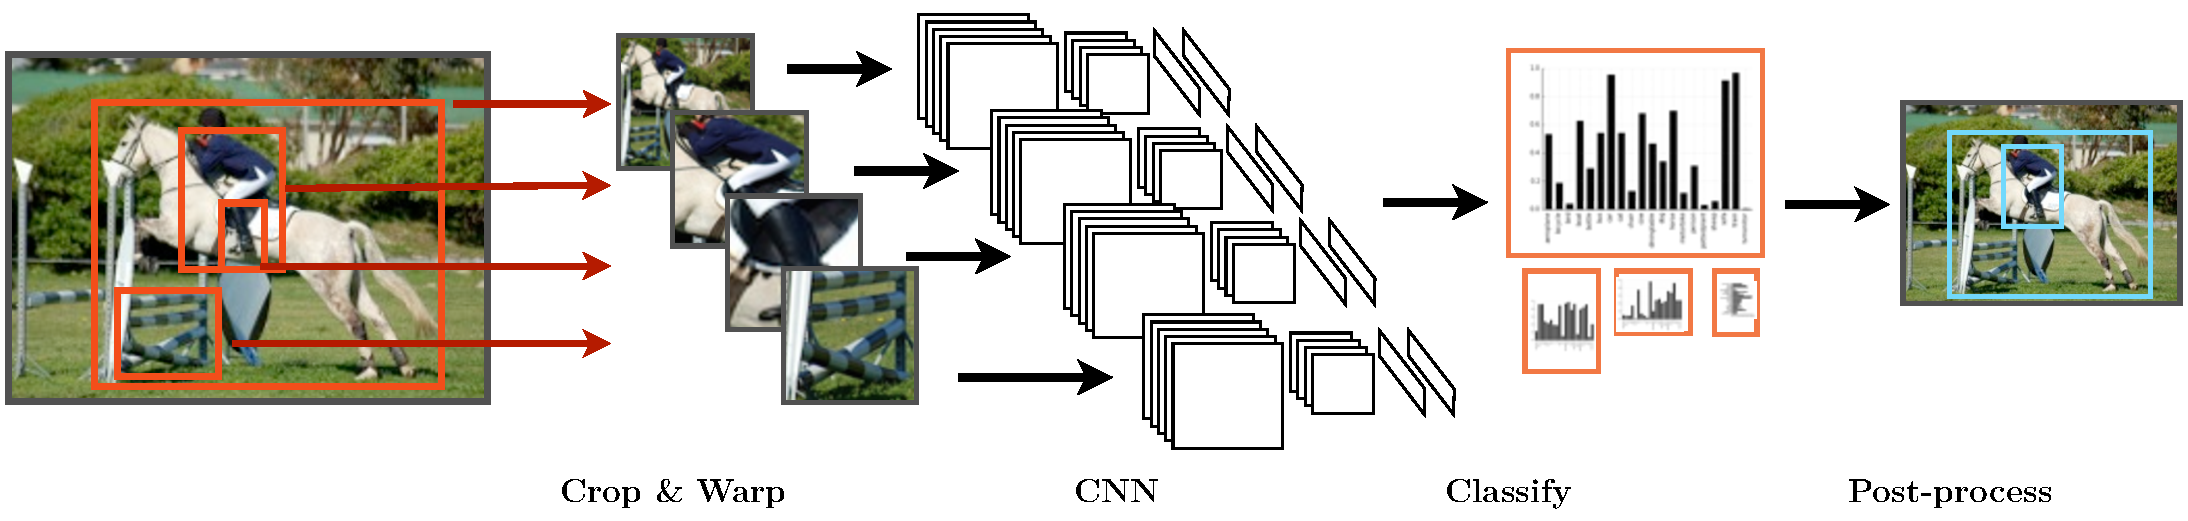
\includegraphics[width=0.98\columnwidth]{../ccnn/figures/rcnn.pdf}
\caption[
Summary of the R-CNN architecture.]{
R-CNN architecture: image regions are cropped, resized, and each one fed through a CNN.
The classifier outputs are post-processed to give the final detections.
}\label{fig:rcnn}
\end{center}
\end{figure}


\begin{figure}[ht]
\begin{center}
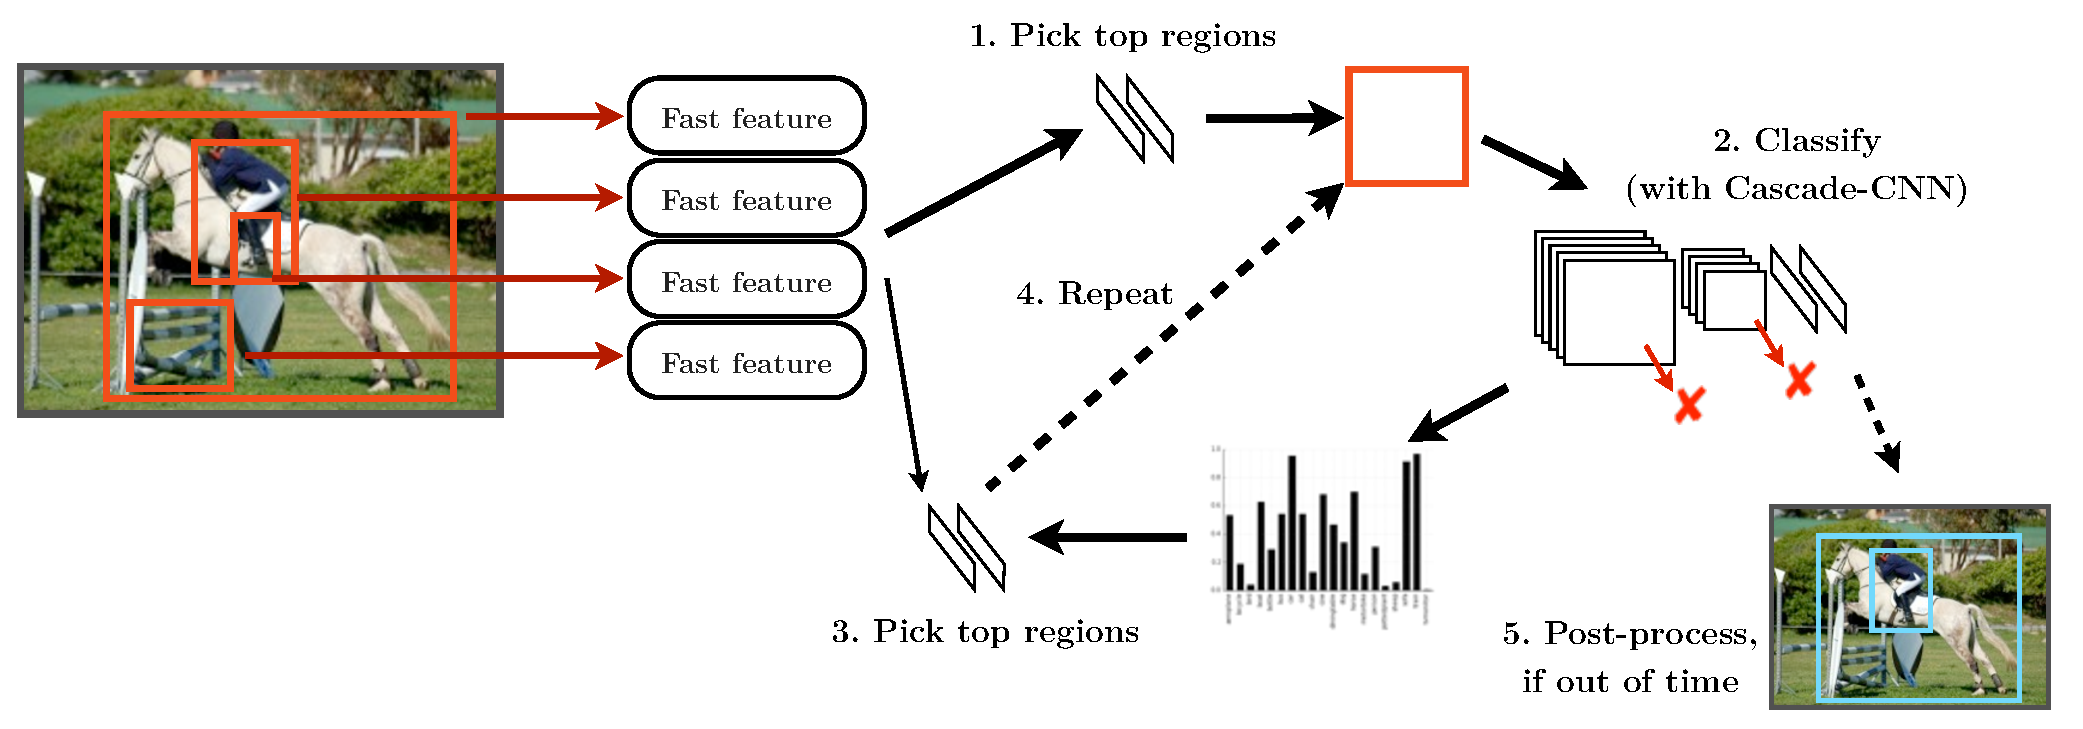
\includegraphics[width=0.98\columnwidth]{../ccnn/figures/combined.pdf}
\caption[
Summary of our method for dynamic region selection and cascaded CNN processing.]{
Our method scores each region of interest with a fast feature (we evaluate several), allowing us to pick promising regions first.
The regions are classified with the original CNN, or a sped-up Cascade-CNN.
The properties of the regions can play a role in selecting the next batch of regions.
}\label{fig:combined}
\end{center}
\end{figure}


\subsection{Quick-to-compute feature}

\PM{Region statistics}
For the first source of information, we consider statistics about ROI location and overlap with other regions.
For each ROI, we compute: its normalized location, its scale ($\sqrt{\text{width} \times \text{height}}$), aspect ratio ($\log \sqrt{\text{width} / \text{height}}$), and normalized counts of overlapping regions, at several PASCAL overlap thresholds (0, 0.2, 0.6).
This simple feature works suprisingly well for filtering regions to process first.

\PM{Pixel gradient}
In concatenation, we also consider the \emph{pixel gradient}, back-propagated throgh a classification CNN applied to the whole image.
This feature corresponds to a kind of saliency map, giving an estimate of the importance of each pixel to the final classification of the image.
Our method is independently developed, but agrees with the concurrently published work of \cite{Simonyan-ICLR-2014} quite closely.
Images are resized to square and classified with an ``AlexNet'' \cite{Krizhevsky-NIPS-2012} CNN fine-tuned on the PASCAL VOC classification dataset with multi-label loss.
(Unlike the ILSVRC, the PASCAL VOC is a multi-label prediction task, with at times multiple correct labels for an image.)
At test-time, the gradient at the top is with respect to the indicator function of the max-scoring class, and is back-propagated all the way to the pixels, where it is summed across channels.
A couple of example images are shown in \autoref{fig:gradient_examples}.
We compute an integral image on this pixel gradient map, allowing near-instant computation of sums in arbitrary regions.
For each region to be evaluated, we compute the image-normalized gradient sum, sums for each of four corners, and ratio of in-region vs. out-of-region sums.

\begin{figure}
\centering
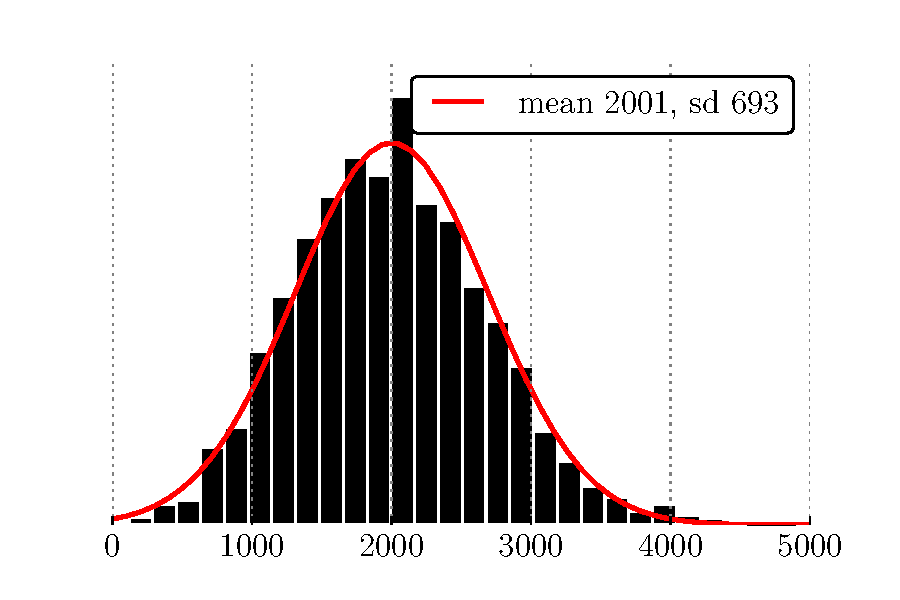
\includegraphics[width=.66\linewidth]{../ccnn/figures/roi_hist.pdf}
\caption{
Distribution of number of regions per image.
}\label{fig:roi_hist}
\end{figure}

\begin{figure}
\centering
\includegraphics[width=.66\linewidth]{../../figures/gradient_backprop.pdf}
\caption[Explanation of the gradient back-propagation quick feature.]{
As a quick feature, we back-propagate the gradient from the top classification layer all the way to the input pixels.
This induces a kind of saliency map on the image, which is useful signal for selecting image sub-regions to classify with the CNN.
}\label{fig:gradient_examples}
\end{figure}

\subsection{Cascade CNN}\label{sec:ccnn}

\PM{Motivation}
Despite the intentions of the region-proposal mechanism \parencite{Uijlings-IJCV-2013}, most ROIs that are scored in R-CNN do not contain any object of interest.
As in the classic cascade of \cite{Viola-IJCV-2004}, it would be useful to quickly reject these regions, without expending the full amount of computation on them.
The problem is that the deep neural network architecture is trained to always run all the way through.
We need to introduce a new primitive to enable early termination.

\PM{Method}
The Cascade CNN, shown in \autoref{fig:ccnn}, augments the CNN network with an ``Early Reject'' option: after some layers, the network decides whether to keep processing the input with the next layer.
Each reject layer is implemented as a fully-connected layer following a linear rectification, trained with dropout using logistic loss on foreground/background labels.
We first train an AlexNet-architecture network \parencite{Krizhevsky-NIPS-2012} on the ImageNet classification dataset.
This network is augmented with the Reject layers, its loss replaced with a multi-label cross-entropy loss, and fine-tuning on the PASCAL VOC training set is performed until loss stop decreasing (roughly 50000 iterations).
In training, all instances pass through all Reject layers.
After training, we set the reject thresholds to maintain at last 80\% recall at each stage, using a large sample of regions from images in the validation set containing positive and negative examples in equal proportion.

\PM{Implementation}
In the efficient implementation of CNNs we use (Caffe), there is a simple loop over each batch element in both CPU and GPU convolution code.
We modify this loop to simply not perform convolution on those elements that were rejected earlier in the cascade.
\footnote{While memory remains occupied in this scheme, we do not consider this a problem.}
Since most of the time is spent in the convolutional layers, we introduce a reject option after \texttt{pool1}, \texttt{pool2}, and \texttt{conv3}.
The last classification layer still outputs the full multi-class scores for the surviving regions.

\PM{Timing}
To estimate the saving on time by using the rejectors we timed the time spend to process 1000 regions (10 batches or 100) and the time expended in each of the first 3 layers:
\begin{itemize}
\item 1700 ms to process all the layers
\item 270 ms (15\%) in layer 1 (This includes \texttt{conv1}, \texttt{relu1}, \texttt{pool1}, \texttt{norm1})
\item 360 ms (20\%) in layer 2 (This includes \texttt{conv2}, \texttt{relu2}, \texttt{pool2}, \texttt{norm2})
\item 285 ms (15\%) in layer 3 (This includes \texttt{conv3}, \texttt{relu3})
\end{itemize}
Therefore the expected ``lifetimes'' of regions rejected after layer 1, layer 2, and layer 3 are  0.15, 0.35, and 0.5 of the total time taken per region.

\begin{figure}[h!]
\begin{center}
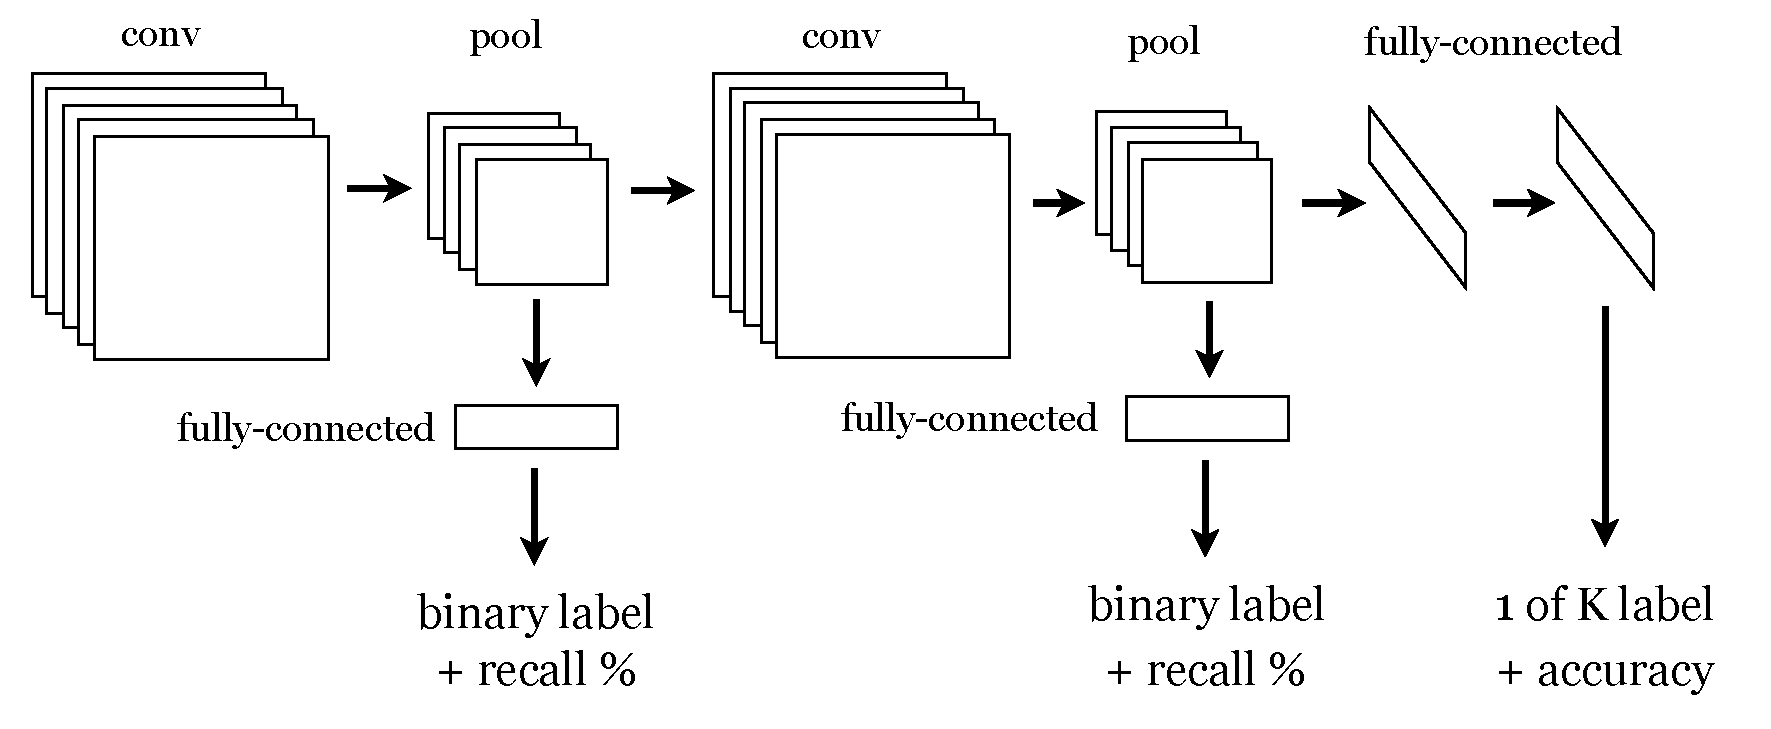
\includegraphics[width=0.98\columnwidth]{../ccnn/figures/ccnn-expanded.pdf}
\caption{
The Cascade CNN has a Reject option after computationally expensive layers, implemented as a binary prediction for reject/keep (background/foreground for our detection task).
The goal of the Reject layer is to maintain high recall while culling as much of the batch as possible, so that we can avoid doing as much convolution in the next layer.
}\label{fig:ccnn}
\end{center}
\end{figure}



%!TEX root=../paper/paper.tex
\section{Evaluation}\label{sec:ccnn_evaluation}

\PM{Dataset}
We evaluate on the standard object detection benchmark: the PASCAL VOC \cite{pascal-voc-2010}.
In all cases, the CNN region classifiers are trained on the PASCAL VOC 2007 trainval set.
The parameters of our methods are set by training or cross-validation on the VOC 2007 val set.
We evaluate on the VOC 2007 test set.
The result plots and details are shown in \autoref{fig:voc2007_results} and \autoref{tab:ccnn_results}.

\PM{Implementation}
The scoring function for the quick-to-compute features is trained by a logistic regression classifier onto the max PASCAL overlap with any ground truth window on the validation dataset.
The classifier is optimized by stochastic gradient descent, and its regularization parameter is cross-validated.
The R-CNN software was used as available in June 2014.
\footnote{\url{https://github.com/rbgirshick/rcnn}}
That software relies on Selective Search \cite{Uijlings-IJCV-2013} region proposals.
Different images are proposed different numbers of regions.
\autoref{fig:roi_hist} shows the distribution of number of regions on the validation set, with the parameters of the R-CNN.
An additional parameter is the size of each batch of regions that goes through the CNN.
We set batch size to 100 regions, and observe that it takes on average 500 ms to process them with the CNN.
In all experiments, we use Ubuntu 12.04, Intel i5 3.2GHz CPU, and NVIDIA Tesla K40 GPU.

%!TEX root=../paper/paper.tex
\begin{figure}[ht]
\begin{subfigure}[b]{\linewidth}
    \centering
    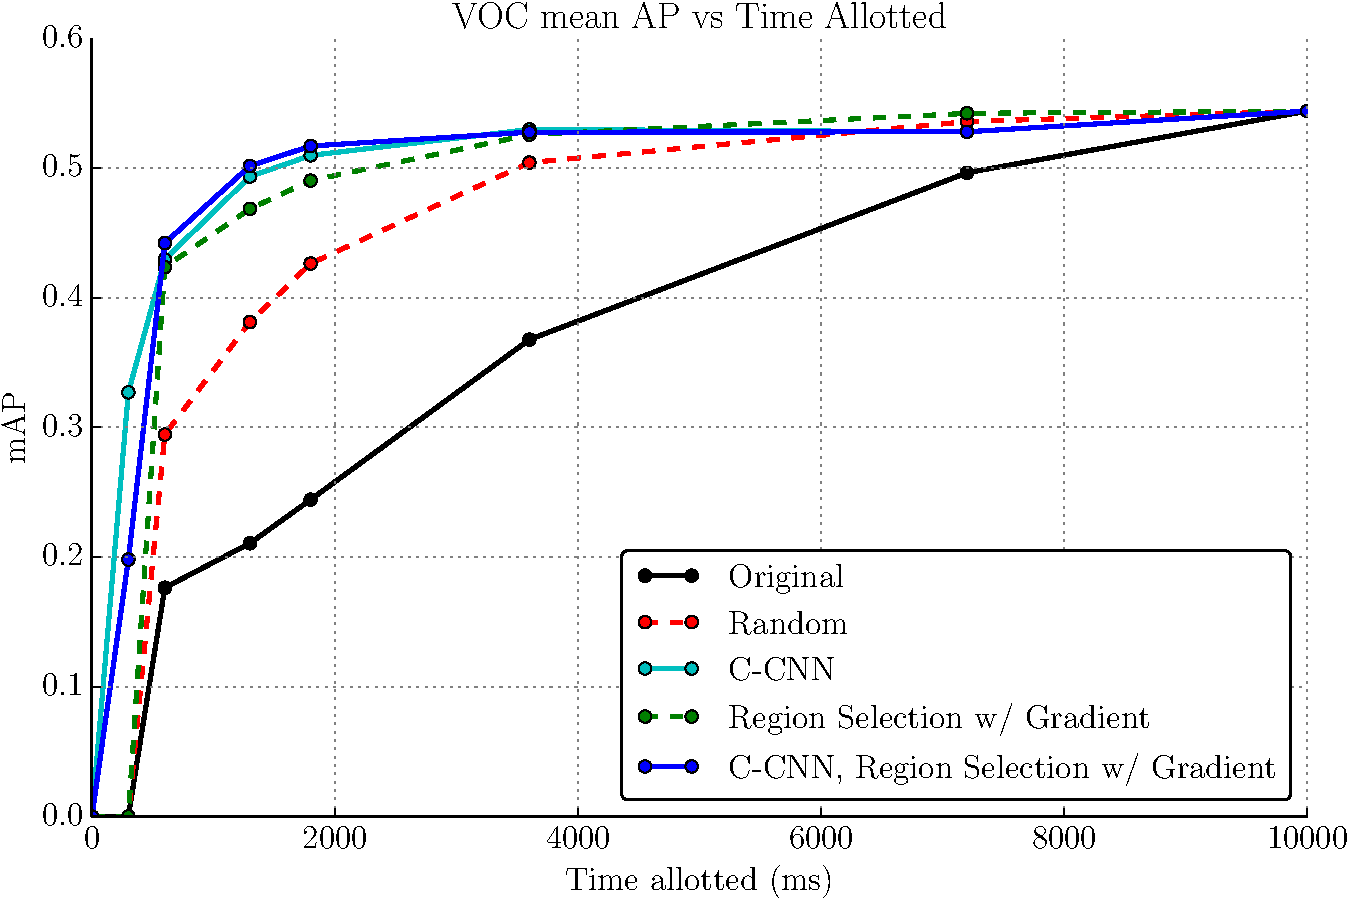
\includegraphics[width=.75\linewidth]{../ccnn/figures/_apvst_final.pdf}
    \caption{
Plotting Mean AP vs. Time Allotted allows comparison performance at a given time budget.
For example, at 1300 ms, random region selection gets about 0.42 mAP, while our best method (C-CNN with gradient-based region selection) obtains 0.50 mAP.
}\label{fig:apvst}
\end{subfigure}
\begin{subfigure}[b]{\linewidth}
    \centering
    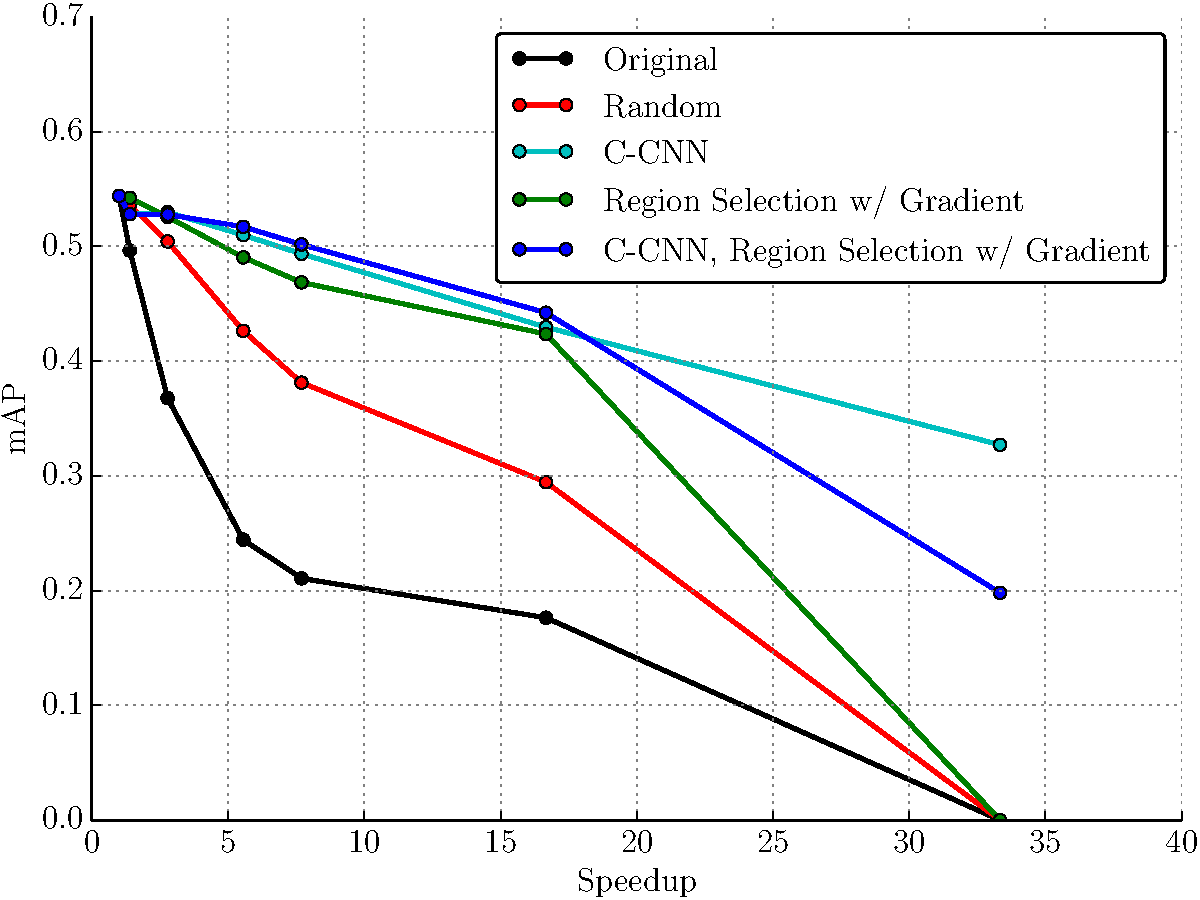
\includegraphics[width=.75\linewidth]{../ccnn/figures/_speedup_final_abs.pdf}
    \caption{
Plotting mean AP vs. speed-up factor allows comparison of speed-ups at a given mAP point.
For example, we can see that we should obtain mAP of 0.40 at around 20x speedup with our method.
}\label{fig:speedup}
\end{subfigure}
\caption{
Results of the Cascade CNN and other Anytime methods on the PASCAL VOC 2007 dataset.
}\label{fig:voc2007_results}
\end{figure}


\begin{table}[ht]
\centering
\caption{
Full table of AP vs. Time results on PASCAL VOC 2007.
Best performance for each time point is in bold.
}\label{tab:ccnn_results}
\small{
\begin{tabular}{lrrrrrrrr}
\toprule
Time allotted (ms)                  & 0 & 300            & 600            & 1300           & 1800           & 3600           & 7200           & 10000 \\
\midrule
Original                            & 0 & 0.000          & 0.176          & 0.211          & 0.244          & 0.368          & 0.496          & 0.544 \\
Random                              & 0 & 0.000          & 0.295          & 0.381          & 0.426          & 0.504          & 0.536          & 0.544 \\
C-CNN                               & 0 & \textbf{0.327} & 0.430          & 0.493          & 0.510          & 0.528          & 0.528          & - \\
Region Selection w/ Gradient        & 0 & 0.000          & 0.424          & 0.469          & 0.490          & 0.526          & \textbf{0.542} & 0.544 \\
C-CNN, Region Selection w/ Gradient & 0 & 0.198          & \textbf{0.442} & \textbf{0.502} & \textbf{0.517} & \textbf{0.528} & 0.528          & - \\
\bottomrule
\end{tabular}
}
\end{table}


The experimental settings are
\begin{description}
  \item[Original] \hfill \\
  The original order of the Selective Search regions of interest.
  This order is influenced by the hierarchical segmentation of their method, and so has sequences of highly overlapping regions.

  \item[Random] \hfill \\
  A completely blind permutation of the original order.

  \item[Region Selection] \hfill \\
  The region statistics feature is always used.
  Additionally, we consider the Pixel Gradient feature, with \emph{setup time} of the gradient forward-back propagation of 20 ms.

  \item[Cascade CNN] \hfill \\
  The Cascade CNN model, as described in \autoref{sec:ccnn}.
  The first experiment (C-CNN) takes batches of regions in a random order.
  The next two experiments also make use of the Region Selection methodology with the quick-to-compute feature.
\end{description}

\PM{Analysis}
Since the time to process a full batch with a non-Cascade CNN is 500 ms, there are no results for non-cascaded baselines at 300 ms.
At this time, the Cascade CNN without any region ordering is best.
A reason for why C-CNN with Region Selection is not as good at this point is that the region selection presents better region candidates, with fewer rejection opportunities, and thus has less coverage of the image.
At 600 ms, C-CNN method have had more than one batch go through, and the Region Selection is giving it a lead over the simple C-CNN.
Both method are better than the baseline non-cascaded methods for this entire duration.


%!TEX root=paper/paper.tex
\chapter{Reinforcement Learning for Anytime Classification}\label{sec:clf_chapter}

\PM{Motivation}
In the previous chapter, running a detector was a very costly action.
In other settings, such as classification problems, we may want to efficiently select a subset of fast features to compute.
For Anytime performance, we should be able to effectively classify any subset of features our policy selects.

%!TEX root=paper/paper.tex
\section{Problem definition}\label{sec:clf_problem}

\begin{mydef} \label{def:clf_problem}
\textbf{The test-time efficient multi-class classification problem} consists of

\begin{itemize}
    \item $N$ instances labeled with one of $K$ labels: ${\mathcal{D} = \{x_n \in \mathcal{X}, y_n \in \mathcal{Y} = \{1, \dots, K\}\}_{n=1}^N}$.
    \item $F$ features $\mathcal{H} = \{h_f : \mathcal{X} \mapsto \mathbb{R}^{d_f} \}_{f=1}^F$, with associated costs $c_f$.
    \item Budget-sensitive loss $\mathcal{L}_\mathcal{B}$, composed of cost budget $\mathcal{B}$ and loss function ${\ell(\hat{y}, y) \mapsto \mathbb{R}}$.
\end{itemize}

The goal is to find a \textbf{feature selection} policy $\pi(x): \mathcal{X} \mapsto 2^\mathcal{H}$ and a \textbf{feature combination} classifier $g(\mathcal{H}_\pi) : 2^\mathcal{H} \mapsto \mathcal{Y}$ such that such that the total budget-sensitive loss $\sum \mathcal{L}_\mathcal{B}(g(\pi(x_n)), y_n)$ is minimized.
\end{mydef}

\PM{Budget}
The cost of a selected feature subset $\mathcal{H}_{\pi(x)}$ is $C_{\mathcal{H}_\pi(x)}$.
The budget-sensitive loss $\mathcal{L}_\mathcal{B}$ presents a hard budget constraint by only accepting answers with $C_{\mathcal{H}} \leq \mathcal{B}$.
Additionally, $\mathcal{L}_\mathcal{B}$ can be \textbf{cost-sensitive}: answers given with less cost are more valuable than costlier answers.
As discussed in \autoref{sec:introduction}, the motivation for the latter property is Anytime performance; we should be able to stop our algorithm's execution at any time and have the best possible answer.

\PM{Cost}
Feature costs $c_f$ can be specified flexibly, with options including theoretical analysis, number of flops, wall clock runtime, total CPU time, or exact power expenditure.
We believe that a deployment in a modern datacenter is most likely to optimize for power expenditure.
In the absence of reliable ways to measure power, we use total CPU time to define the cost: if an operation is performed in parallel on multiple cores, its cost is considered to be the total cpu time on all cores.

\PM{Shared features}
The features $h_f$ can be classifier outputs, possibly multi-class; following convention, we refer to such features as \emph{weak learners}.
For a weak learner $h_f$, the cost $c_f$ is composed of the cost of an underlying feature extraction $\phi_{h_f}(x)$ and the cost of subsequent classification.
Once $h_f$ is computed, its underlying feature $\phi$ is considered to be free for all other features $h_f'$ that share it, if any, such that $c_f' < c_f$.
Note that in state-of-the-art object recognition systems, complex features and feature encodings are often followed by linear classifiers, and feature extraction cost dominates the total cost.

\begin{figure}[ht]
\centering
\includegraphics[width=.85\linewidth]{../../figures/feature_selection_sequence.pdf}
\caption[
Summary of our dynamic feature selection approach to the classification problem.]{
We model the problem of state traversal as a Markov Decision Process.
For every state, we learn to select action of maximum expected value.
The state is updated with the result of the selected action.
We train a classifier on subsets of features, to give answer at any time.
}\label{fig:feature_selection_sequence}
\end{figure}


\PM{Train vs. test}
At training time, our computation is unbudgeted, and we can compute all features to have \emph{fully-observed} training instances.
At test time, there is a budget and so the instances we classify will only be \emph{partially-observed}, as determined by the feature selection policy.
\autoref{fig:feature_selection_sequence} shows the sequential process we are learning.


%!TEX root=paper/paper.tex
\section{Method}\label{sec:clf_method}

\PM{MDP summary}
We model the \textbf{feature selection} policy $\pi(x): \mathcal{X} \mapsto 2^\mathcal{A}$ following the reinforcement learning approach as described in \autoref{sec:mdp_formulation}.
The set of \textbf{actions} $\mathcal{A}$ is exactly the set of features $\mathcal{H}$.
The policy learning approach remains the same, including implementation details.
In summary, we learn the $\theta$ by \emph{policy iteration}.
First, we gather $(s, a, r, s')$ samples by running episodes (to completion) with the current policy parameters $\theta_i$.
From these samples, $\hat{Q}(s, a)$ values are computed, and $\theta_{i+1}$ are given by $L_2$-regularized least squares solution to $\hat{Q}(s, a) = \theta^T \phi(s, a)$, on all states that we have seen in training.

\PM{Classifier}
Three things are different: the reward definition, the state featurization function, and the additional dependence on a classifier.
We defer discussion of learning the \textbf{feature combination} classifier $g(\mathcal{H}_\pi) : 2^\mathcal{H} \mapsto \mathcal{Y}$ to~\autoref{sec:clf_classifier}.
For now, we assume that $g$ can combine an arbitrary subset of features and provide a distribution $P(Y = y)$.
For example, $g$ could be a Naive Bayes (NB) model trained on the fully-observed data.

%!TEX root=paper/paper.tex
\subsection{Reward definition}\label{sec:clf_reward}

\input{../clf_rewards_fig}

\PM{Loss vs. cost}
The budget-sensitive loss $\mathcal{L}_\mathcal{B}$ enforces Anytime performance by valuing early gains more than later gains.
To formalize this, consider \autoref{fig:clf_rewards}, which shows the entropy and the 0-1 loss of $g$ at every point in a sequential feature selection episode for some instance $x$.
For the best Anytime performance, we want to capture the most area above the loss vs. cost curve, up to max budget $\mathcal{B}$.
Recall from \eqref{eq:expected_reward} that the value of an episode $\xi$ is defined as the sum of obtained rewards.
If the reward of a single action is defined as the area above the curve that is captured as a direct result, then the value of the whole episode exactly corresponds to $\mathcal{L}_\mathcal{B}$.

\PM{Infogain}
However, there is a problem with using loss directly: only the first action to ``tip the scale'' toward the correct prediction gets a direct reward (in the figure, it is the first action).
A smoother reward function is desirable: if the classifier $g$ can give a full distribution $P(Y = y \mid \mathcal{H}_{\pi(x)})$ and not just a prediction $\hat{y} \in \mathcal{Y}$, we can maximize the \emph{information gain} of the selected subset instead of directly minimizing the loss of $g(\pi(x))$:
\begin{eqnarray}
I(Y; \mathcal{H}_{\pi(x)}) &=& H(Y) - H(Y | \mathcal{H}_{\pi(x)}) = \\ \notag
&=& \sum_{y \in Y} P(y) \log P(y) - \\ \notag
&&\sum_{y, \mathcal{H}_{\pi(x)}} P(y, \mathcal{H}_{\pi(x)}) \log P(y \mid \mathcal{H}_{\pi(x)})
\end{eqnarray}

\PM{Definition}
To the extent that $g$ is unbiased, maximizing information gain corresponds to minimizing loss, and ensures that we not only make the right classification decision but also become maximally certain.
Therefore, as graphically presented in \autoref{fig:clf_rewards}, we define the reward of selecting feature $h_s$ with cost $c_f$ with the set $\mathcal{H}_s$ computed to be $I_{\mathcal{H}_s}(Y; h_f) (\mathcal{B}_s - \frac{1}{2}c_f)$.
Although we do not evaluate in this regime, note that this definition easily incorporates a \textbf{setup cost} in addition to \textbf{deadline cost} by only computing the area in between setup and deadline costs.


%!TEX root=paper/paper.tex
\subsection{Features of the state}\label{sec:clf_features}

The featurization function $\phi(s)$ extracts the following features from the state:

\begin{itemize}\addtolength{\itemsep}{-.5\baselineskip}
\item Bit vector $\textbf{m}$ of length $F$: initially all bits are $1$ and are set to $0$ when the corresponding feature is computed.
\item For each $h_f$, a vector of size $d_f$ representing the values; $0$ until observed.
\item Cost feature $c \in [0, 1]$, for fraction of the budget spent.
\item Bias feature $1$.
\end{itemize}

\PM{Static vs Dynamic}
These features define the \textbf{dynamic} state, presenting enough information to have a \emph{closed-loop} (dynamic) policy that may select different features for different test instances.
The \textbf{static} state has all of the above features except for the observed feature values.
This enables only an \emph{open-loop} (static) policy, which is exactly the same for all instances.
Policy learned with the static state is used as a baseline in experiments.


%!TEX root=paper/paper.tex
\subsection{Learning the classifier}\label{sec:clf_classifier}

\PM{Classifiers}
We have so far assumed that $g$ can combine an arbitrary subset of features and provide a distribution $P(Y = y)$---for example, a Gaussian Naive Bayes (NB) model trained on the fully-observed data.
However, a Naive Bayes classifier suffers from its restrictive independence assumptions.
Since discriminative classifiers commonly provide better performance, we'd like to use a \textbf{logistic regression} classifier.
Nearest Neighbor methods also provide a robust classifier for partially observed data, but are slow for large datasets.
We consider them in this exposition and in preliminary experiments reported in \autoref{sec:imputation_evaluation}, but do not use them in final policy learning experiments due to this problem.

\PM{Missing features}
Note that at test time, some feature values are missing.
If the classifier is trained exclusively on fully-observed data, then the feature value statistics at test time will not match, resulting in poor performance.
Therefore, we need to learn classifier weights on a distribution of data that exhibits the pattern of missing features induces by the policy $\pi$, and/or try to intelligently impute unobserved values.

\input{../clf_algorithm}

\PM{Joint learning}
At the same time, learning the policy depends on the classifier $g$, used in the computation of the rewards.
For this reason, the policy and classifier need to be learned jointly: \autoref{alg:learning} gives the iterative procedure.
In summary, we start from random $\pi$ and $g$, gather a batch of trajectories.
The batch is used to update both $g$ and $\pi$.
Then new trajectories are generated with the updated $\pi$, rewards are computed using the updated $g$, and the process is repeated.

\subsubsection{Unobserved value imputation}

\PM{Formulation}
Unlike the Naive Bayes classifier, the logistic regression classifier is not able to use an arbitrary subset of features $\mathcal{H}_\pi$, but instead operates on feature vectors of a fixed size.
To represent the feature vector of a fully observed instance, we write $\mathbf{x} = [h_1(x), \dots, h_f(x)]$.
In case that $\mathcal{H}_\pi \subset \mathcal{H}$, we need to fill in unobserved feature values in the vector.

\PM{Formulation}
We can think of the policy as a test-time feature selection function $o(x, b): \mathcal{X} \times \mathbb{R} \mapsto \mathbb{B}^F$, where $\mathbb{B} \in \{0, 1\}$, and $b \in [0, 1]$ is given and specifies the fractional selection \emph{budget}.
Applied to $x$, $o(x, b)$ gives the binary selection vector $\mathbf{o}$ which splits $\mathbf{x}$ it into observed and unobserved parts such that $\mathbf{x}^m = [\mathbf{x}^\text{o}, \mathbf{x}^\text{u}]$.
$X^c$ denotes the fully observed $N \times F$ training set.
We assume that we have only sequential access to the missing-feature test instances $\mathbf{x}^m$.

\PM{Mean imputation}
A basic strategy is \textbf{mean imputation}: filling in with the mean value of the feature.
We simply replace the missing value in $X^m$ with their row mean in $X^c$.
Because our data is always zero-mean, this amounts to simply replacing the value with $0$.
\begin{align}
\mathbf{x}_\pi = \left[ h_i(x) : \left\{ \begin{array}{rl}
 h_i(x) &\mbox{ if $h_i \in \mathcal{H}_{\pi(x)}$} \\
 \bar{\mathbf{h}}_i &\mbox{ otherwise}
\end{array} \right. \right]
\end{align}

\PM{Gaussian Imputation}
If we assume that $\mathbf{x}$ is distributed according to a multivariate Gaussian $\mathbf{x} \sim \mathcal{N}(\mathbf{0}, \Sigma)$, where $\Sigma$ is the sample covariance $X^T X$ and the data is standardized to have zero mean, then it is possible to do \textbf{Gaussian imputation}.
Given a feature subset $\mathcal{H}_\pi$, we write:
\begin{equation}
\mathbf{x}_\pi = \begin{bmatrix} \mathbf{x}^\text{o}\\  \mathbf{x}^\text{u} \end{bmatrix} \sim \mathcal{N} \left( \mathbf{0}, \begin{bmatrix} \mathbf{A} & \mathbf{C}\\ \mathbf{C}^T & \mathbf{B} \end{bmatrix} \right)
\end{equation}
where $\mathbf{x}^\text{o}$ and $\mathbf{x}^\text{u}$ represent the respectively observed and unobserved parts of the full feature vector $\mathbf{x}$, $\mathbf{A}$ is the covariance matrix of (here and elsewhere, the part of $X^c$ corresponding to) $\mathbf{x}^\text{o}$, $\mathbf{B}$ is the covariance matrix of $\mathbf{x}^\text{u}$, and $C$ is the cross-variance matrix that has as many rows as the size of $\mathbf{x}^\text{o}$ and as many columns as the size of $\mathbf{x}^\text{u}$ \parencite{Roweis-gaussian-identities}.
In this case, the distribution over unobserved variables conditioned on the observed variables is given as
$\mathbf{x}^\text{u} \mid \mathbf{x}^\text{o} \sim \mathcal{N} \left( \mathbf{C}^T \mathbf{A}^{-1} \mathbf{x}^\text{o},\, \mathbf{B} - \mathbf{C}^T \mathbf{A}^{-1} \mathbf{C} \right)$.

\PM{Complexity}
After computing the complete covariance matrix $\Sigma$, which takes $O(N^3)$ time, we need to make $N'$ test-time predictions.
In the course of the predictions, we may need to compute at most $\min(N', 2^F)$ unique matrix inversions (again in $O(N^3)$).
The size of the matrices being inverted is proportional to the budget $b$, making this method slower for larger budgets.

\PM{k-NN Imputation and Prediction}
Instead of assuming anything, we could go directly to the source of the covariances---the actual feature values for all points in the training set.
The family of Nearest Neighbor methods takes this approach.
The algorithm for imputation is simple: find the nearest neighbors in the observed dimensions, and use their averaged values to fill in the unobserved dimensions.
For $\mathbf{X}^m$, we find the $k$ nearest neighbors with the highest dot product similarity $\mathbf{x}^{cT} \mathbf{x^m}$ or lowest Euclidean distance $\| \mathbf{x}^{c} - \mathbf{x}^{m} \|$, using only the features that are observed in $\mathbf{x}^{m}$.
For \textbf{imputation}, the unobserved values are set to the average across these nearest neighbors for that dimension.
Similarly, we do \textbf{classification} by returning the mode label of the nearest neighbors.

\PM{Complexity}
Finding the nearest neighbors by dot product similarity is $O(NF'^2)$, and Euclidean distance is the same with an additional constant term.
$F'S$ is the number of observed dimensions, which grows proportionally with budget $b$, making this method more expensive with increased budget.

\subsubsection{Learning more than one classifier}

\input{../mdp_masks_fig}

\PM{Subset clustering}
As illustrated in \autoref{fig:mdp_masks}, the policy $\pi$ selects some feature subsets more frequently than others.
Instead of learning only one classifier $g$ that must be robust to all observed feature subsets, we can learn several classifiers, one for each of the most frequent subsets.
This is done by maintaining a distribution over encountered feature subsets during training.

We use hierarchical agglomerative clustering, growing clusters bottom-up from the observed masks.
In the case of training $K$ classifiers, we need to find $K$ clusters such that the masks are distributed as evenly as possible into the clusters.
The distance measure for the binary masks is the Hamming distance; standard K-Means clustering technique is not applicable to this distance measure.
Each one of $K$ classifiers is trained with the \textsc{Liblinear} implementation of logistic regression, with $L_2$ regularization parameter K-fold cross-validated at each iteration.



%!TEX root=paper/paper.tex
\section{Evaluation}\label{sec:clf_evaluation}

\PM{Settings}
We evaluate the following sequential selection baselines:

\begin{itemize}
\item \textbf{Static, greedy}: corresponds to best performance of a policy that does not observe feature values and selects actions greedily ($\gamma=0$).
\item \textbf{Static, non-myopic}: policy that does not observe feature values but uses the MDP machinery with $\gamma=1$ to consider future action rewards.
\item \textbf{Dynamic, greedy}: policy that observed feature values, but selects actions greedily.
\end{itemize}

Our method is the \textbf{Dynamic, non-myopic} policy: observed feature values, and full lookahead.

\PM{Metrics}
We evaluate two forms of test-time efficient performance measure: the area under the curve and the performance at max budget.
(Note that all methods are trained only for the former measure.)

\PM{Classifier}
In preliminary experiments, Logistic Regression always performed better than the Gaussian Naive Bayes classifier, and so only the former is used in the experiments below.
We evaluated classification with \textbf{Gaussian} vs. \textbf{Mean} imputation, and with different number of classifiers (1, 3, and 6) clustered by feature subsets.
We found that Gaussian imputation performed better than mean imputation, but not substantially, and at additional cost.
Although increased number of classifiers sometimes increased performance, it also made our method prone to overfitting.
In the final accounting, $K=1$ classifiers worked best on all tasks.
Results of detailed experiments on imputation and clustering are given in \autoref{sec:imputation_evaluation}.
For policy experiments, we report only the best achieved imputation method.

\PM{Details}
For details on the reinforcement learning implementation, see \autoref{sec:mdp_formulation} and \autoref{sec:det_evaluation}.
We largely rely on classifier implementations in the \texttt{scikit-learn} package \parencite{Pedregosa2011}.
With pre-computed features, our training procedure takes only a few hours on an $8$-core \emph{Xeon E5620} machine for each of the experiments below.

\subsection{Experiment: Synthetic}

\begin{figure*}[ht]
\centering
\includegraphics[width=\linewidth]{../../figures/synthetic_explanation.pdf}
\caption[Setup of the synthetic example.]{
See text for explanation.
}\label{fig:synthetic_setup}
\end{figure*}


\begin{figure*}[ht]
\centering
\includegraphics[width=\linewidth]{../../figures/synthetic_trajectories.pdf}\\
\includegraphics[width=\linewidth]{../../figures/apr11_assembly/synthetic_orthants_D3_False_N16000_Nt4000_13.pdf}
\caption[Evaluation of the classification approach on the synthetic example.]{
Evaluation on the synthetic example (best viewed in color).
The sample feature trajectories of different policies at top: the opacity of the edges corresponds to their prevalence during policy execution; the opacity of the nodes corresponds to the amount of reward obtained in that state.
Note that the \emph{static, non-myopic} policy correctly learns to select the cheap features first, but is not able to correctly branch, while our \emph{dynamic, non-myopic} approach finds the optimal strategy.
The plots in the bottom half give the error vs. cost numbers.
}\label{fig:synthetic_results}
\end{figure*}


\PM{Setup}
Following \cite{Xu-ICML-2013}, we first show that the policy works as advertised in a challenging synthetic example.
In $D$-dimensional space, the data has a label for each of the $2^D$ orthants, and is generated by a unit-variance Gaussian in that orthant (See top left of \autoref{fig:synthetic_setup} for the 3D case).
There are $D$ cheap features that simply return the sign of the data point's coordinate for the corresponding dimension.
For each orthant, there is also an expensive feature that returns the data point's label if the point is located in the corresponding orthant, and random noise otherwise.

\PM{Results}
The optimal policy on a new data point is to determine its orthant with cheap features, and then take the corresponding expensive action.
Note that both dynamic features and non-myopic learning are crucial to the optimal policy, which is successfully found by our approach.
\autoref{fig:synthetic_results} shows the results of this optimal policy, a random policy, and of different baselines and our method, trained given the correct minimal budget.

\subsection{Experiment: Scene recognition}

%!TEX root=paper/paper.tex
\begin{figure*}[ht]
\centering
    \centering
    \begin{subfigure}[b]{0.5\textwidth}
            \includegraphics[width=\textwidth]{../../figures/apr11_assembly/scene_15_5_crop.pdf}
            \caption{Error given by policies learned for a budget = 5.}
    \end{subfigure}%
    \begin{subfigure}[b]{0.44\textwidth}
            \includegraphics[width=\textwidth]{../../figures/apr11_assembly/_scenes15_auc.pdf}
            \caption{Areas under error vs. cost curves of policies learned at different budgets.}
    \end{subfigure}\\
    \begin{subfigure}[b]{0.47\textwidth}
            \includegraphics[width=\textwidth]{../../figures/apr11_assembly/scene15_5/static.pdf}
            \caption{Trajectory of our static policy.}
    \end{subfigure}%
    \begin{subfigure}[b]{0.47\textwidth}
            \includegraphics[width=\textwidth]{../../figures/apr11_assembly/scene15_5/dynamic.pdf}
            \caption{Trajectory of our dynamic policy.}
    \end{subfigure}\\
    \caption[Results of the classification approach on the Scenes-15 dataset.]{
Results on Scenes-15 dataset (best viewed in color).
Figure (a) shows the error vs. cost plot for policies learned given a budget of 5 seconds.
Figure (b) aggregates the area under the error vs. cost plot metrics for different policies and budgets, showeing that our approach outperforms baselines no matter what budget it's trained for.
Figures (d) and (e) shows the branching behavior of our dynamic policy vs the best static policy.
}\label{fig:clf_scenes}
\end{figure*}


\PM{Setup}
The Scene-15 dataset \parencite{Lazebnik-CVPR-2006} contains 4485 images from 15 visual scene classes.
The task is to classify images according to scene.
Following \parencite{Xiao-CVPR-2010}, we extracted 14 different visual features (GIST, HOG, TinyImages, LBP, SIFT, Line Histograms, Self-Similarity, Textons, Color Histograms, and variations).
The features vary in cost from 0.3 seconds to 8 seconds, and in single-feature accuracy from 0.32 (TinyImages) to .82 (HOG).
Separate multi-class linear SVMs were trained on each feature channel, using a random 100 positive example images per class for training.
We used the \texttt{liblinear} implementation, and K-fold cross-validated the penalty parameter $C$.
The trained SVMs were evaluated on the images not used for training, resulting in a dataset of 2238 vectors of 210 confidence values: 15 classes for each of the 14 feature channels.
This dataset was split 60-40 into training and test sets for our experiments.

\PM{Results}
\autoref{fig:clf_scenes} shows the results, including learned policy trajectories.
For all evaluated budgets, our \emph{dynamic, non-myopic} method outperforms all others on the area under the error vs. cost curve metric.
Our results on this dataset match the reported results of Active Classification \parencite{Gao-NIPS-2011} (Figure 2) and Greedy Miser \parencite{Xu-ICML-2012} (Figure 3), although both methods use an additional powerful feature channel (ObjectBank)\footnote{Detailed results for this and other experiments are on the project page (see front page for the \href{http://sergeykarayev.com/recognition-on-a-budget/}{link}).}.

\subsection{Experiment: ImageNet and maximizing specificity}

%%!TEX root=paper/paper.tex
\begin{figure}[ht]
\centering
\includegraphics[width=\linewidth]{../../figures/imagenet_tree.pdf}
\caption[The ImageNet recognition challenge structures object categories in a DAG.]{
    The ImageNet recognition challenge structures object categories in a DAG.
    Here we show the whole structure and highlight a few sub-categories.
    (Figure courtesy of Yangqing Jia.)
}\label{fig:imagenet_tree}
\end{figure}


\PM{Setup}
The full ImageNet dataset has over 10K categories and over a million images \parencite{Deng-ECCV-2010}.
% \autoref{fig:imagenet_tree} shows the hierarchical organization of the dataset.
The classes are organized in a hierarchical structure, which can be exploited for novel recognition tasks.
We evaluate on a 65-class subset introduced in ``Hedging Your Bets'' \parencite{Deng-CVPR-2012}.
In this evaluation, we consider the situation where the initial feature computation has already happened, and the task is to find a path through existing one-vs-all classifiers: features correspond to Platt-scaled SVM confidences of leaf-node classifiers (trained on SIFT-LLC features), and each has cost 1 \parencite{Deng-ECCV-2010}.
Following \parencite{Deng-CVPR-2012}, accuracy is defined on all nodes, and inner node confidences are obtained by summing the probabilities of the descendant nodes.

\PM{Results}
We combine our sequential feature selection with the ``Hedging Your Bets'' method for backing off prediction nodes using the ImageNet hierarchy to maintain guaranteed accuracy while giving maximally specific answers, given a cost budget.
The results are given in \autoref{fig:imagenet}.
As the available budget increases, the \emph{specificity} (defined by normalized information gain in the hierarchy) of our predictions also increases, while accuracy remains constant.
Visualizing this on the ILSVRC-65 hierarchy, we see that the fraction of predictions at the leaf nodes grows with available computation time.
This formulation presents a novel angle on modeling the time course of human visual perception.

\begin{figure*}[ht]
\centering
    \begin{subfigure}[b]{0.52\textwidth}
            \includegraphics[width=\textwidth]{../../figures/apr11_assembly/_ilsvrc65_auc.pdf}
            \caption{
            Areas under error vs. cost curves for policies learned at different budgets.
            (No specificity back-off is performed here).
            \label{fig:imagenet-a}
            }
    \end{subfigure}\hfill%
    \begin{subfigure}[b]{0.43\textwidth}
            \includegraphics[width=\textwidth]{../../figures/apr11_assembly/ilsvrc65_acc.pdf}
            \caption{
            Holding prediction accuracy constant, we achieve increased specificity with increased cost (on \emph{Dynamic, non-myopic} policy, budget = 36).
            \label{fig:imagenet-b}
            }
    \end{subfigure}\\\vspace{1em}
    \begin{subfigure}[b]{.97\textwidth}
            \includegraphics[width=\textwidth]{../../figures/apr11_assembly/ilsvrc65_network-crop.pdf}
            \caption{
            We visualize the fraction of predictions made at inner vs. leaf nodes of ILSVRC-65 at different cost points of an Anytime policy: with more computation, accurate predictions are increasingly made at the leaf nodes.
            \label{fig:imagenet-c}
            }
    \end{subfigure}
\caption[Results of the classification approach on the ILSVRC-65 dataset.]{
Results on the ILSVRC-65 dataset (best viewed in color).
Figure (a) shows our dynamic approaches outperforming static baselines for all practical cost budgets.
When our method is combined with Hedging Your Bets \parencite{Deng-CVPR-2012}, a constant prediction accuracy can be achieved at all points in the Anytime policy, with \emph{specificity} of predictions increasing with the cost of predictions.
Figures (b) and (c) show this for the \emph{dynamic, non-myopic} policy learned for budget = 26.
This is analogous to human visual performance, which shows increased specificity at longer stimulus times.
}\label{fig:imagenet}
\end{figure*}



%!TEX root=paper/paper.tex
\chapter{Conclusion}\label{sec:conclusion}

\PM{Main Contribution}
We note a significant problem that has received little research attention: Anytime visual recognition.
The problem is motivated by the properties of human visual perception and by the need to effectively schedule computationally expensive state-of-the-art computer vision methods for different computational budgets.
We approach the problem from the perspective of reinforcement learning, and successfully learn fully general policies for selecting detector and classifier actions.
To evaluate our approaches, we introduce a new metric of Anytime performance, based on the area under the performance vs. cost curve.
In all experiments, we show that having a dynamic state (and thus allowing ``closed-loop'' policies) and planning ahead increases performance.

\PM{Detection}
We present a method for learning closed-loop policies for multi-class object detection, given existing object detectors and classifiers and a metric to optimize.
The method learns the optimal policy using reinforcement learning, by observing execution traces in training.
As with most reinforcement learning problems, the reward function is defined manually, with domain knowledge.
Here, we derive it for the novel detection AP vs. Time evaluation that we suggest is useful for evaluating efficiency in recognition.
If detection on an image is cut off after only half the detectors have been run, our method does $66\%$ better than a random ordering, and $14\%$ better than an intelligent baseline.
In particular, our method learns to take action with no intermediate reward in order to improve the overall performance of the system.

\PM{Classification}
For the classification task, we need to use a different inference mechanism and additionally need to train classifiers for partially-observed sets of features.
We investigate methods such as different forms of imputation and classifier clustering for this task, and adjust the reward function and the featurization of the state.
Using our method, we show improved Anytime performance on a synthetic classification task and two benchmark visual recognition tasks.
Furthermore, on a hierarchically-structured dataset, we show that accuracy of predictions can be held constant for all budgets, while the specificty of predictions increases.

\PM{Anytime CNN Detection}
Even the most recent state-of-the-art CNN-based detection methods are computationally expensive.
We first consider approaches which can effectively reorder the sequence of regions to maximize the chance that correct detections will be found early, based on inference from relatively lightweight features.
We show that basic strategies, such as simply reordering the boxes such that they do not have a degenerate spatial layout, provides a surprising boost, and that very simple features such as region and gradient statistics can effectively prioritize regions.
Our main contribution is the Cascade CNN model, which adds a novel Reject layer between convolutional layers in the architecture.
C-CNN obtains an 8x speedup of the R-CNN detection method with only a 10\% degradation of state-of-the-art performance on PASCAL VOC detection.

\PM{Recognizing Style}
We have also made significant progress in defining the problem of recognizing image style.
We provide a novel dataset of several types of visual style -- including for visual art -- not previously considered in the literature.
In preparation for an Anytime approach, we evaluate several types of visual features on the dataset, and demonstrate state-of-the-art results in prediction of both style and aesthetic quality (on an existing dataset).
We confirm that our results are comparable to human performance, show that style is highly content-dependent, and demonstrate an image search application where results are queried by content and filtered by style.

\section{Future Work}

\subsection{Detection and Classification}

\PM{Decision Cost}
Computation devoted to scheduling actions is far less significant than the computation due to running the actions in all of our work, and our framework does not explicitly consider this decision-making cost.
However, a welcome extension would explicitly model the decision cost by drawing on existing theoretical work on meta-reasoning (such as \cite{Hay2012}).
Interesting extensions could try to balance the cost of inference vs. the expected gain in efficiency.

\PM{NN Methods}
Nearest-neighbor methods are well suited to settings with partially observed sets of features, and so could be a good addition to our work on Anytime classification.
However, naive NN methods are too slow for our purposes, and we did not evaluate them.
Locality-sensitive hashing methods such as \cite{Kulis2009b} may be an effective solution.
In particular, the original method of \cite{Gao-NIPS-2011} could potentially be extended with hashing to maintain its model-free advantages over a rigidly parametrized model at an acceptable speed.

\PM{Perception}
Beyond the aspects of practical deployment of vision systems that our work is motivated by, we are curious to further investigate our model as a tool to study human cognition and the time course of visual perception.
Only a few attempts have been made to explain this: for example, via sequential decision processes in \textcite{Hegde-Neuro-2008}.
While we have not made any claims about the biological mechanism of perception, our work in reinforcement learning-based feature selection as well as convolutional neural networks has explanatory potential if more tightly integrated in future work.

\PM{Adaptive Submodularity}
The most intriguing future direction is in theoretical analysis of our Anytime method.
Our MDP-based formulation is empirically successful, but fundamentally heuristic.
Adaptive submodularity \parencite{Golovin-and-Krause-2010-JAIR}, a recently developed framework for obtaining famous near-optimality results of \cite{Nemhauser1978} in the context of learning policies.
Just as that work proved that greedy selection can be near-optimal if some conditions of the set function are satisfied, \cite{Golovin-and-Krause-2010-JAIR} prove that greedy policies can also be near-optimal under certain conditions.
Unfortunately, designing an appropriate objective function for our task of visual recognition is not straightforward.

\PM{Submodular Ideas}
Information gain, a component of our reward function, can be shown to not be submodular \cite{Krause-UAI-2005}, so the easy solution has a roadblock.
The most promising way forward is pointed by recent work on active learning and robotic grasping.
In \cite{Golovin-2010}, an adaptively submodular objective based on hypothesis space pruning is developed for an active learning task.
In \cite{Javdani2012}, robotic grasping is linked to a submodular set cover problem --- and another set cover analogy is developed in \cite{Chen-2014-ICML} for the problem of picking computer vision detections to evaluate with an oracle.
An adaptively submodular objective for the general classification problem seems close.
Alternatively, we could show that our reward function is empirically submodular -- but that is not as interesting.

\subsection{CNN-based recognition}

\PM{Cascade CNN}
The general structure of the Cascade CNN general structure of simply ``thinning'' input batches as they travel through the network is agnostic to the underlying mechanism.
Although in our work we evaluate on the R-CNN method on the PASCAL dataset, the Cascade CNN can be applied to the SPP-net method of \cite{He-ECCV-2014}, or the part-based method of \cite{Zhang-ECCV-2014}.
In fact, the Cascade CNN can be applied to any existing CNN that predicts in a class-imbalanced domain where speed is important --- speech recognition, for example.

\PM{End-to-end}
Although, the Cascade CNN is shown to be a strong method for speeding up CNN-based detection approaches, its layers were trained in a stage following the initial network training, not in an \emph{end-to-end} fashion that is the hallmark of deep learning models.
Furthermore, the thresholds were set in a separate process, using a special validation set.
Future work should train and set thresholds of the Reject layers at the same time as the other layers are trained, not after the fact.

\begin{figure}[h!]
\begin{center}
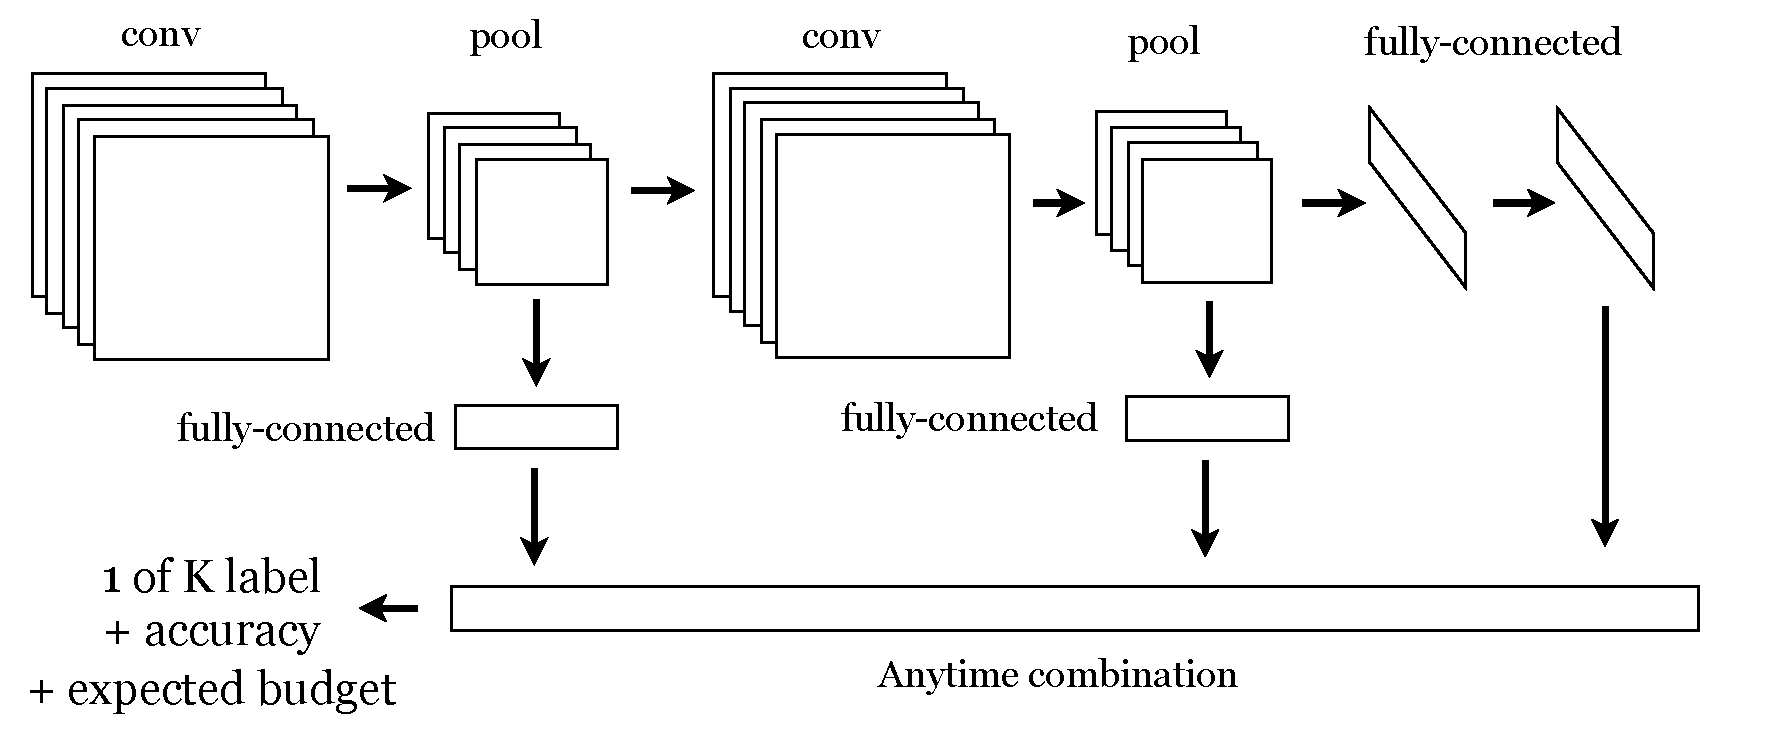
\includegraphics[width=0.98\columnwidth]{../ccnn/figures/ccnn-expanded-anytime.pdf}
\caption[Architecture of the proposed Anytime CNN.]{
The proposed Anytime CNN augments traditional networks with fully-connected prediction layers after every computationally-expensive layer.
All prediction layers feed into an Anytime combination layer that computes accuracy and back-propagates from cost-sensitive loss.
Compare this architecture to \autoref{fig:ccnn}.
}\label{fig:ccnn_anytime}
\end{center}
\end{figure}


\PM{Anytime loss}
More interestingly, networks could be augmented with an ``Anytime loss'' layer that combines classification output from multiple levels of the network in a cost-sensitive way.
This would allow optimizing classification networks for arbitrary distributions of cost budgets.
\autoref{fig:ccnn_anytime} shows the idea: the new layer combines the outputs of all fully-connected layers, which are regularly placed throughout the network.
The Anytime loss computes the expected accuracy of each prediction, takes into account the computational cost up to that layer of the network, and back-propagates according to the budget (for example, if no answers are allowed after 50 ms, and it takes 60 ms to get through the network fully, then the final fully connected layer predictions are never counted).
This setup allows for modeling a distribution over budgets.

\subsection{Image Style}
\PM{Anytime}
While we collected two datasets and showed first results on the challenging new task of recognizing image style, we did not evaluate Anytime performance of our features.
Part of the reason was that one of the most interesting outcomes of this work was the success of features trained on object categorization datasets, and in particular the CNN-based feature.
Although we make a separate Anytime contribution to the CNN in \autoref{sec:ccnn_chapter}, it would still be interesting to evaluate Anytime performance of other visual features on the style datasets.

\PM{Features}
We propose several possible hypotheses to explain the success of general multi-layer features on the style dataset, despite not having been trained on the style task.
Perhaps the network layers that we use as features are extremely good as general visual features for image representation in general.
Another explanation is that object recognition depends on object appearance, e.g., distinguishing red from white wine, or different kinds of terriers, and that the model learns to repurpose these features for image style.
Understanding and improving on these results is fertile ground for future work.

%!TEX root=paper/paper.tex
\chapter{Reinforcement Learning for Anytime Detection}\label{sec:det_chapter}

%!TEX root=paper/paper.tex
\section{Problem Definition}\label{sec:det_problem}

\begin{figure}[ht]
\centering
\includegraphics[width=\linewidth]{../../../2011-2012/figures/figure1.pdf}
\caption[A sample trace of our Anytime sequential process detection method.]{
A sample trace of our method.
At each time step beginning at $t=0$, potential actions are considered according to their predicted \emph{value}, and the maximizing action is picked.
The selected action is performed and returns \emph{observations}.
Different actions return different observations: a detector returns a list of detections, while a scene context action simply returns its computed feature.
The \emph{belief model} of our system is updated with the observations, which influences the selection of the next action.
The final evaluation of a detection episode is the area of the \emph{AP vs. Time} curve between given start and end times.
The value of an action is the expected result of final evaluation if the action is taken and the policy continues to be followed, which allows actions without an immediate benefit to be scheduled.
}\label{fig:det_figure1}
\end{figure}


\PM{Definitions}
We deal with a dataset of images $\mathcal{D}$, where each image $x$ contains zero or more objects.
Each object is labeled with exactly one category label $k \in \{1, \dots, K\}$.
The multi-class, multi-label \textbf{classification} problem asks whether $x$ contains at least one object of class $k$.
We write the ground truth for an image as $\mathbf{C}=\{C_1, \dots, C_K\}$, where $C_k \in \{0, 1\}$ is set to $1$ if an object of class $k$ is present.
The \textbf{detection} problem is to output a list of bounding boxes (sub-images defined by four coordinates), each with a real-valued confidence that it encloses a single instance of an object of class $k$.
The answer for a single class $k$ is given by an algorithm $\emph{detect}(x,k)$, which outputs a list of sub-image bounding boxes $B$ and their associated confidences.

\PM{Evaluation metric}
Performance is evaluated by plotting precision vs. recall across dataset $\mathcal{D}$ (by progressively lowering the confidence threshold for a positive detection).
The area under the curve yields the Average Precision (AP) metric, which has become the standard evaluation for recognition performance on challenging datasets in vision \parencite{pascal-voc-2010}.
A common measure of a correct detection is the PASCAL overlap: two bounding boxes are considered to match if they have the same class label and the ratio of their intersection to their union is at least $\frac{1}{2}$.
Multi-class performance is evaluated by averaging the individual per-class AP values.
In a specialized system such as the advertising case study from~\autoref{sec:introduction}, the metric generalizes to a weighted average, with the weights set by the \emph{values} of the classes.

\PM{Policy}
Our goal is a multi-class recognition policy $\pi$ that takes an image $x$ and outputs a list of multi-class detection results by running detector and global scene \emph{actions} sequentially.
The policy repeatedly selects an action $a_i \in \mathcal{A}$, executes it, receiving observations $o_i$, and then selects the next action.
The set of actions $\mathcal{A}$ can include both classifiers and detectors: anything that would be useful for inferring the contents of the image.

\PM{Actions}
Each action $a_i$ has an expected cost $c(a_i)$ of execution.
Depending on the setting, the cost can be defined in terms of algorithmic runtime analysis, an idealized property such as number of \emph{flops}, or simply the empirical runtime on specific hardware.
We take the empirical approach: every executed action advances $t$, the \emph{time into episode}, by its runtime.
The specific actions we consider in the following exposition are detector actions $a_{{det}_i}$, where ${det}_i$ is a detector class $C_i$, and a scene-level context action $a_{gist}$, which updates the probabilities of all classes.
Although we do not showcase this here, note that our system easily handles multiple detector actions per class.

\PM{Anytime metric}
As shown in \autoref{fig:det_figure1}, the system is given two times: the setup time $T_s$ and deadline $T_d$.
We want to obtain the best possible answer if stopped at any given time between the setup time and the deadline.
A single-number metric that corresponds to this objective is the area captured under the curve between the start and deadline bounds, normalized by the total area.
We evaluate policies by this more robust metric and not simply by the final performance at deadline time for the same reason that Average Precision is used instead of a fixed Precision vs. Recall point in the conventional evaluations.
Additionally, maximizing this single-number metric corresponds to maximizing Anytime performance.


%!TEX root=paper/paper.tex
\section{Method}\label{sec:det_method}

%!TEX root=paper/paper.tex
\subsection{MDP Formulation}\label{sec:mdp_formulation}

To model the \textbf{action selection} policy $\pi(x): \mathcal{X} \mapsto 2^\mathcal{A}$, we employ the Markov Decision Process (MDP) to model a single \emph{episode} of selecting actions for some instance $x$.

\begin{mydef} \label{def:MDP}
The \textbf{feature selection MDP} consists of the tuple $(\mathcal{S}, \mathcal{A}, T(\cdot), R(\cdot), \gamma)$:

\begin{itemize}
\item \textbf{State} $s \in \mathcal{S}$ stores the selected action subset $\mathcal{A}_{\pi(x)}$, resulting observations, and total cost $C_{\mathcal{A}_{\pi(x)}}$.
\item The set of \textbf{actions} $\mathcal{A}$.
\item The \textbf{state transition} distribution $T(s' \mid s, a)$ can depend on the instance $x$.
\item The \textbf{reward} function $R(s, a, s') \mapsto \mathbb{R}$ is manually specified, and depends on the actions taken and the instance $x$.
\item The discount $\gamma$ determines amount of \textbf{lookahead} in selecting actions: if 0, actions are selected greedily based on their immediate reward; if 1, the reward accrued by subsequent actions is given just as much weight as the reward of the current action.
\end{itemize}
\end{mydef}

\PM{Trajectories and reward}
A recognition \emph{episode} takes an image $\mathcal{I}$ and proceeds from the initial state $s^0$ and action $a^0$ to the next pair $(s^1,a^1)$, and so on until $(s^J,a^J)$, where $J$ is the last step of the process with $t \le T_d$.
At that point, the policy is terminated, and a new episode can begin on a new image.
We call this a \emph{trajectory} $\xi = (s_0, a_0, s_1, r_1, \dots, a_{I-1}, s_I, r_I)$, where $I$ is the total number of actions taken (and therefore features selected), $s_0$ is the initial state, $a_i \sim \pi(a \mid s_i)$ is chosen by the \emph{policy} $\pi(a \mid s)$, and $s_{i+1} \sim T(s \mid s_i, a_i)$, which can depend on $x$.
The total expected reward (value) of an MDP episode is written as
\begin{equation}\label{eq:expected_reward}
V_\pi(s_0) =
\mathbb{E}_{\xi \sim \left\{ \pi, x \right\}} r(\xi) =
\mathbb{E}_{\xi \sim \left\{ \pi, x \right\}} \left[ \sum_{i=0}^I \gamma^i \, r_i \right]
\end{equation}

\PM{Q-Value function}
We seek $\pi$ that maximizes \autoref{eq:expected_reward}.
If we had a function accurately predicting the value of taking an action in a state, we could define the policy as simply taking the action with maximum value from any state.
We specify this function $Q(s,a): S \times \mathcal{A} \mapsto \mathbb{R}$, where $S$ is the space of all possible states, to assign a value to a potential action $a \in \mathcal{A}$ given the current state $s$ of the decision process.
We can then define the policy $\pi$ as simply $\argmax_{a_i \in \mathcal{A} \setminus \mathcal{O}} Q(s,a_i)$.
The Q-function is defined and learned recursively:
\begin{align}\label{eq:recursive_value}
Q^\pi(s^j,a) = \mathbb{E}_{s^{j+1}} [R(s^j,a) + \gamma Q^\pi(s^{j+1},\pi(s^{j+1}))]
\end{align}

\subsection{Learning the policy}
\PM{Function approximation}
Although the action space $\mathcal{A}$ is manageable, the space of possible states $S$ is intractable, and we must use function approximation to represent $Q(s,a)$: a common technique in reinforcement learning \parencite{Sutton1998}.
We featurize the state-action pair and assume linear structure:
\begin{align}\label{eq:policy}
Q^\pi(s,a) = \theta_\pi^\top \phi(s,a)
\end{align}
where $\phi: \mathcal{S} \times \mathcal{A} \mapsto \mathbb{R}^{d_s}$ is the state featurization function, $d_s$ is the dimensionality of the state feature vector, and $\theta^\pi$ is a vector of weights that defines the policy $\pi$.

\PM{Policy function}
Specifically, the policy is defined as
\begin{equation}
\pi(a \mid s) = \frac{1}{Z} \exp\left(\frac{1}{\tau} \theta^T \phi(s, a)\right)
\end{equation}
where $Z$ is the appropriate normalization and $\tau$ is a temperature parameter that controls the level of exploration vs. exploitation in the policy.
As $\tau \rightarrow 0$, ${\pi(a \mid s)}$ becomes highly peaked at $\argmax_a Q(s,a)$; it becomes uniform as $\tau \rightarrow \infty$.
In training, this parameter is turned down gradually.

\input{../qiteration_explanation_fig}

\PM{Sampling Q-function}
While we can't directly compute the expectation in \autoref{eq:recursive_value}, we can sample it by running actual episodes to gather $<s,a,r,s'>$ samples, where $r$ is the reward obtained by taking action $a$ in state $s$, and $s'$ is the following state.
We then learn the optimal policy by repeatedly gathering samples with the current policy, minimizing the error between the discounted reward to the end of the episode as predicted by our current $Q(s^j,a)$ and the actual values gathered, and updating the policy with the resulting weights.
This method is akin to fitted Q-iteration, a variant of generalized policy iteration \parencite{Ernst2005,Sutton1998}.
\autoref{fig:qiteration_explanation} shows a step of this process.

\PM{Gathering trajectories}
During training, we gather samples starting from either a random feasible state, with probability $\epsilon$, or from the initial empty state otherwise.
Both $\epsilon$ and $\tau$ parameters decay exponentially with the number of training iterations.
Training is terminated if $\pi_{\theta_{i+1}}$ returns the exact same sequence of episodes $\xi$ on a validation set as $\pi_{\theta_{i}}$.
During test time, $\epsilon$ is set to $0.05$.

\PM{Block-coding}
To formulate learning the policy as a single regression problem, we could represent the features in block form, where $\phi(s,a)$ is a vector of size $F|\mathcal{A}|$, with all values set to $0$ except for the $F$-sized block corresponding to $a$.
An implementation detail: instead of block-coding $\phi(s,a)$, we learn $F$ separate $\theta_f$'s for the features $\phi(s)$: one for each action $a$
To prevent overfitting, we use $L_2$-regularized regression.
The weight $\alpha$ of the regularization term is tied across the $F$ separate regressions and is tuned by cross-validation on 3 folds.

\PM{Details}
We run $15$ iterations of accumulating samples by running $350$ episodes, starting with a baseline policy which will be described in \autoref{sec:det_evaluation}, and cross-validating the regularization parameter at each iteration.
Samples are not thrown away between iterations.

\subsubsection{Greedy vs non-myopic}

\PM{Greedy}
Note from \autoref{eq:recursive_value} that the $\gamma \in [0,1]$ parameter of the MDP controls the level of \emph{discounting} of rewards of future action in computing the value \autoref{eq:expected_reward}.
In the baseline \textbf{greedy} setting, with $\gamma=0$, rewards gained by future actions are not counted at all in determining the value of the current action.
The value function is determined entirely by the immediate reward, and so only completely greedy policies can be learned in this case.
This setting is used as baseline.

\PM{Non-myopic}
In the \textbf{non-myopic} setting, with $\gamma=1$, rewards gained by future actions are valued exactly as much as reward gained by the current action in determining its value.
However, a slightly lower value of $\gamma$ mitigates the effects of increasing uncertainty regarding the state transitions over long episodes.
We set this meta-parameter of our approach through cross-validation, and find that a mid-level value ($0.4$) works best.


\begin{figure}[ht]
\centering
\includegraphics[width=\linewidth]{../../../2011-2012/figures/pomdp_annotated.pdf}
\caption[Summary of our closed-loop action selection method for Anytime detection.]{
Our closed-loop method consists of selecting an action based on the belief state, executing action almost as a ``black box,'' which makes our method very general, and then updating the state with the received observations.
}\label{fig:pomdp_summary}
\end{figure}


Our sequential method is visually summarized in \autoref{fig:pomdp_summary}.

%!TEX root=paper/paper.tex
\subsection{Reward definition}\label{sec:det_reward}

\PM{AP of state}
The policy's performance at time $t$ is determined by all detections that are part of the set of observations $\mathbf{o}^j$ at the last state $s^j$ before $t$.
Recall that detector actions returns lists of detection hypotheses.
Therefore, the final AP vs. Time evaluation of an episode is a function $eval(h,T_s,T_d)$ of the history of execution $h=s^0,s^1,\dots,s^J$.
It is precisely the normalized area under the AP vs. Time curve between $T_s$ and $T_d$, as determined by the detections in $\mathbf{o}^j$ for all steps $j$ in the episode.

\PM{Additive rewards}
Note from Figure~\ref{fig:det_rewards} that this evaluation function is additive per action, as each action $a$ generates observations that may raise or lower the mean AP of the results so far ($\Delta ap$) and takes a certain time ($\Delta t$).
We can accordingly represent the final evaluation $eval(h,T_s,T_d)$ in terms of individual action rewards: $\sum_{j=0}^J R(s^j,a^j)$.
Specifically, as shown in Figure~\ref{fig:det_rewards}, we define the \emph{reward} of an action $a$ as

\begin{align}\label{eq:det_reward}
R(s^j,a) = \Delta \text{ap} (t_T^j-\frac{1}{2}\Delta t)
\end{align}

where $t_T^j$ is the time left until $T_d$ at state $s^j$, and $\Delta t$ and $\Delta \text{ap}$ are the time taken and AP change produced by the action $a$.
(We do not account for $T_s$ here for clarity of exposition.)


%!TEX root=paper/paper.tex
\subsection{Features of the state}\label{sec:det_features}

\PM{State}
We refer to the information available to the decision process as the \emph{state} $s$.
The state includes the current estimate of the distribution over class presence variables $P(\mathbf{C}) = \{P(C_0), \ldots, P(C_K)\}$, where we write $P(C_k)$ to mean $P(C_k=1)$ (class $k$ is present in the image).
Additionally, the state records that an action $a_i$ has been taken by adding it to the initially empty set $\mathcal{O}$ and recording the resulting observations $o_i$.
We refer to the current set of observations as $\mathbf{o} = \{o_i | a_i \in \mathcal{O}\}$.
The state also keeps track of the time into episode $t$, and the setup and deadline times $T_s,T_d$.

\PM{Open vs Closed Loop}
An \emph{open-loop} policy, such as the common classifier cascade \parencite{Viola-IJCV-2004}, takes actions in a sequence that does not depend on observations received from previous actions.
In contrast, as presented in \autoref{fig:pomdp_summary}, our goal is to learn a dynamic, or \emph{closed-loop}, policy, which would exploit the signal in scene and inter-object context for a maximally efficient path through the actions.
Recall from \autoref{eq:policy} that our policy is determined by a linear function of the features of the state.

\PM{Dynamic features}
Since we want to be able to learn a dynamic policy, the observations $\mathbf{o}$ that are part of the state $s$ should play a role in determining the value of a potential action.
We include the following quantities as features $\phi(s,a)$:

\begin{tabularx}{0.8\linewidth}{p{0.23\linewidth}p{0.69\linewidth}}
$P(C_a)$ & The prior probability of the class that corresponds to the detector of action $a$ (omitted for the scene-context action).\\
$P(C_0|\mathbf{o}) \ldots P(C_K|\mathbf{o})$ & The probabilities for all classes, conditioned on the current set of observations.\\
$H(C_0|\mathbf{o}) \ldots H(C_K|\mathbf{o})$ & The entropies for all classes, conditioned on the current set of observations. \\
\end{tabularx}

Additionally, we include the mean and maximum of $[H(C_0|\mathbf{o}) \ldots H(C_K|\mathbf{o})]$, and $4$ time features that represent the times until start and deadline, for a total of $F = 1+2K+6$ features.

\PM{Augmented MDP}
Our system as any system of interesting complexity, runs into two related limitations of MDPs: the state has to be functionally approximated instead of exhaustively enumerated; and some aspects of the state are not observed, making the problem a Partially Observed MDP (POMDP), for which exact solution methods are intractable for all but rather small problems \parencite{Roy2002}.
Our initial solution to the problem of partial observability is to include features corresponding to our level of uncertainty into the feature representation, as in the technique of \emph{augmented} MDPs \parencite{Kwok2004}.

\subsubsection{Updating with observations}\label{sec:det_features_updating}

\PM{Class correlations}
The bulk of our feature representation is formed by probability of individual class occurrence, conditioned on the observations so far: $P(C_0|\mathbf{o}) \ldots P(C_K|\mathbf{o})$.
This allows the action-value function to learn correlations between presence of different classes, and so the policy can look for the most probable classes given the observations.
However, higher-order co-occurrences are not well represented in this form.
Additionally, updating $P(C_i|\mathbf{o})$ presents choices regarding independence assumptions between the classes.

\PM{Update methods}
We evaluate two approaches for updating probabilities: \emph{direct} and \emph{MRF}.
In the \emph{direct} method, $P(C_i|\mathbf{o}) = score(C_i)$ if $\mathbf{o}$ includes the observations for class $C_i$ and $P(C_i|\mathbf{o}) = P(C_i)$ otherwise.
This means that an observation of class $i$ does not directly influence the estimated probability of any class but $C_i$.
The \emph{MRF} approach employs a pairwise fully-connected Markov Random Field (MRF), as shown in \autoref{fig:det_figure1}, with the observation nodes set to $score(C_i)$ appropriately, or considered unobserved.

\PM{Learning MRF}
The graphical model structure is set as fully-connected, but some classes almost never co-occurr in our dataset.
Accordingly, the edge weights are learned with $L_1$ regularization, which obtains a sparse structure \parencite{Lee2006}.
All parameters of the model are trained on fully-observed data, and Loopy Belief Propagation inference is implemented with an open-source graphical model package \parencite{Jaimovich2010}.

\PM{Details}
An implementation detail: $score(C_i)$ for $a_{{det}_i}$ is obtained by training a probabilistic classifier on the list of detections, featurized by the top few confidence scores and the total number of detections.
Similarly, $score(C_i)$ for $a_{gist}$ is obtained by training probabilistic classifiers on the GIST feature, for all classes.



%!TEX root=paper/paper.tex
\section{Evaluation}\label{sec:det_evaluation}

%!TEX root=paper/paper.tex
\begin{figure}[ht]
\centering
\includegraphics[width=.49\linewidth]{../../figures/pascal1.pdf}
\includegraphics[width=.49\linewidth]{../../figures/pascal2.pdf}
\caption{
The PASCAL VOC is an object detection dataset presenting a challenging variety of image and object appearance.
}\label{fig:pascal}
\end{figure}


\PM{Dataset}
We evaluate our system on the multi-class, multi-label detection task, as previously described.
Each detection episode takes an image and outputs detections with associated times, based on the order of actions taken.
We evaluate on a popular detection challenge task: the PASCAL VOC 2007 dataset \parencite{pascal-voc-2010}.
Example images from the dataset are shown in \autoref{fig:pascal}.
This datasets exhibits only a modest amount of class co-occurrence: the ``person'' class is highly likely to occur, and less than $10\%$ of the images have more than two classes.

\PM{Metric}
The final evaluation pools all detections up to a certain time, and computes their multi-class AP per image, averaging over all images.
This is done for different times to plot the AP vs. Time curve over the whole dataset.
Our method of averaging per-image performance follows \parencite{Desai2009}.

\PM{Detector}
For the detector actions, we use one-vs-all cascaded deformable part-model detectors on a HOG featurization of the image \parencite{Felzenszwalb-CVPR-2010}, with linear classification of the list of detections as described in the previous section.
There are $20$ classes in the PASCAL challenge task, so there are $20$ detector actions.
Running a detector on a PASCAL image takes about $1$ second.

\PM{Training}
We learn weights on the training and validation sets, and run our policy on all images in the testing set.
With pre-computed detections on the PASCAL VOC 2007 dataset, our training procedure takes about $4$ hours on an $8$-core \emph{Xeon E5620} machine.

\PM{Settings}
We test three different settings of the start and deadline times.
In the first one, the start time is immediate and execution is cut off at $20$ seconds, which is enough time to run all actions.
In the second one, execution is cut off after only $10$ seconds.
Lastly, we measure performance between $5$ seconds and $15$ seconds.
These operating points show how our method behaves when deployed in different conditions.
The results are given in rows of \autoref{tab:det_results}.

\begin{figure}[h!]
\centering
\begin{subfigure}[b]{.48\linewidth}
\includegraphics[width=\linewidth]{../../../2011-2012/figures/apvst_expl.pdf}
\caption{
    Graphical representation of the reward function.
}\label{fig:det_rewards}
\end{subfigure}
%
\begin{subfigure}[b]{.48\linewidth}
\includegraphics[width=\linewidth]{../../../2011-2012/figures/final1_515.png}
\caption{
    AP vs. Time curves for Random, Oracle, the Fixed Order baseline, and our best-performing policy.
}\label{fig:det_results1}
\end{subfigure}
\end{figure}


\PM{Baselines}
We establish the first baseline for our system by selecting actions randomly at each step.
As shown in \autoref{fig:det_results1}, the \textbf{Random} policy results in a roughly linear gain of AP vs. time.
This is expected: the detectors are capable of obtaining a certain level of performance; if half the detectors are run, the expected performance level is half of the maximum level.
To establish an upper bound on performance, we plot the \textbf{Oracle} policy, obtained by re-ordering the actions at the end of each detection episode in the order of AP gains they produced.
We consider another baseline: selecting actions in a fixed order based on the value they bring to the AP vs. Time evaluation, which is roughly proportional to their occurrence probability.
We refer to this as \textbf{Fixed Order}.

\PM{Ours}
Then there are instantiations of our method, as described in the previous section : \textbf{RL w/ Direct} inference and \textbf{RL w/ MRF} inference.
As the \textbf{MRF} model consistently outperformed \textbf{Direct} by a small margin, we report results for that model only.
In additional to the detector actions, we include a scene-level GIST feature that updates the posterior probabilities of all classes.
This is considered one action, takes about $0.3$ seconds, and brings another boost in performance.
The results are shown in \autoref{tab:det_results}.

\begin{figure}[h!]
\centering
\includegraphics[width=\linewidth]{../../../2011-2012/figures/trajectories.pdf}
\caption[
Visualizing action trajectories of different object detection policies.]{
Visualizing the action trajectories of different policies.
Action selection traces are plotted in orange over many episodes; the size of the blue circles correspond to the increase in AP obtained by the action.
We see that the \textbf{Random} policy selects actions and obtains rewards randomly, while the \textbf{Oracle} policy obtains all rewards in the first few actions.
The \textbf{Fixed Order} policy selects actions in a static optimal order.
Our \textbf{RL w/ MRF} policy does not stick a static order but selects actions dynamically to maximize the rewards obtained early on.
}
\label{fig:trajectories}
\end{figure}


\PM{Trajectories}
In \autoref{fig:det_results1}, we can see that due to the dataset bias, the fixed-order policy performs well at first, as the person class is disproportionately likely to be in the image, but is significantly overtaken by our model as execution goes on and more rare classes have to be detected.
It is additionally informative to consider the action trajectories of different policies in \autoref{fig:trajectories}.
In contrast to the fixed order policy, our method is clearly dynamic, jumping from action to action based on the observations obtained from previous actions.

\begin{figure}[h!]
\centering
\begin{subfigure}[t]{.8\linewidth}
    \includegraphics[width=\linewidth]{../../../2011-2012/figures/weights_greedy}
    \caption{Greedy}
\end{subfigure}\\
\begin{subfigure}[t]{.8\linewidth}
    \includegraphics[width=\linewidth]{../../../2011-2012/figures/weights_rl}
    \caption{Reinforcement Learning}
\end{subfigure}
\caption[Learned policy weights for the detection approach.]{
Learned policy weights $\theta_\pi$ (best viewed in color: red corresponds to positive, blue to negative values).
The first row corresponds to the scene-level action, which does not generate detections itself but only helps reduce uncertainty about the contents of the image.
Note that in the greedy learning case, this action is learned to never be taken, but it is shown to be useful in the reinforcement learning case.
}
\label{fig:det_weights}
\end{figure}


\PM{Learned weights}
As an illustration, we visualize the learned weights on features as described in \autoref{sec:det_features} in \autoref{fig:det_weights}.
The weights are reshaped such that each row shows the weights learned for an action, with the top row representing the scene context action and then next $20$ rows corresponding to the PASCAL VOC class detector actions.
We note that the GIST action is learned to never be taken in the greedy ($\gamma=0$) setting, but is learned to be taken with a higher value of $\gamma$.

\begin{table}[t]
\caption{The areas under the AP vs. Time curve for different experimental conditions.}
\label{tab:det_results}
\centering
\begin{tabular}{|c|c|c|c|c|c|}
\hline
Bounds & Random & Fixed Order & RL        & RL w/ GIST         & Oracle \\ \hline
(0,20) & 0.250  & 0.342       & 0.378     & \textbf{0.382}  & 0.488 \\
(0,10) & 0.119  & 0.240       & 0.266     & \textbf{0.267}  & 0.464 \\
(5,15) & 0.257  & 0.362       & 0.418     & \textbf{0.420}  & 0.530 \\ \hline
\end{tabular}
\end{table}


%!TEX root=paper/paper.tex
\chapter{Introduction}\label{sec:introduction}

\section{Motivation}

\PM{Perception}
It is well known that human perception is both Anytime, meaning that a scene can be described after even a short presentation, and progressive, meaning that the quality of description increases with more time.
The progressive time course of visual perception has been confirmed by multiple studies \parencite{Vanrullen-1996,Fei-Fei-Vision-2007}, with some studies providing evidence that enhancement occurs in an ontologically meaningful way.
For example, people tend to recognize something as an animal before recognizing it as a dog \parencite{Mace-PloS-2009}.
The underlying mechanisms of this behavior are not well explored, with only a few attempts made to explain the temporal dynamics --- for instance, a promising work by \cite{Hegde-Neuro-2008} has employed the framework of sequential decision processes.

\PM{Computer applications}
Meanwhile, automated visual recognition has achieved levels of performance that allow useful real-world implementation.
We focus on two problem formulations: \emph{image classification}, in which some property of the image -- such as scene type, visual style, or even object presence -- is predicted, and \emph{object detection}, in which the location and category (or identity) of all objects in a scene is predicted.
Solutions to the two problems are often linked, as classification can be a ``subroutine'' in a detection method.
State-of-the-art methods for classification and detection tend to be computationally expensive, insensitive to Anytime demands, and not progressively enhanced.

\PM{Application}
As real-world deployment of recognition methods grows, managing resource cost (power or compute time) becomes increasingly important.
For tasks such as personal robotics, it is crucial to be able to deploy varying levels of processing to different stimuli, depending on computational demands on the robot.
A hypothetical system for vision-based advertising, in which paying customers engage with the system to have their products detected in images on the internet, presents another example.
The system has different values (in terms of cost per click) and accuracies for different classes of objects, and the backlog of unprocessed images fluctuates based on demand and available server time.
A recognition strategy to maximize profit in such an environment should exploit all signals available to it, and the quality of detections should be Anytime, depending on the length of the queue (for example, lowering recall with increased queue pressure).

\PM{Visual Features \& Classification}
For most state-of-the-art classification methods, a range of features are extracted from an image instance and used to train a classifier.
Since the feature vectors are usually high-dimensional, linear classification methods are used most often.
Features are extracted at different costs, and contribute differently to decreasing classification error.
Although it can generally be said that ``the more features, the better,'' high accuracy can of course be achieved with only a small subset of features for some instances.
Additionally, different instances benefit from different subsets of features.
For example, simple binary features are sufficient to quickly detect faces \parencite{Viola-IJCV-2004} but not more varied visual objects, while the features most useful for separating landscapes from indoor scenes \parencite{Xiao-CVPR-2010} are different from those most useful for recognizing fine distinctions between bird species \parencite{Farrell-ICCV-2011}.
\autoref{fig:features} presents several common visual features.

\PM{Detection}
Detection methods tend to employ the same visual features and classifiers but apply them to many image sub-regions.
Approaches can broadly be grouped into (A) \emph{per-class, all-region}, (B) \emph{all-class, all-region}, and (C) \emph{all-class, proposed-region} methods.
State-of-the-art \emph{all-class, proposed-region} methods such as \cite{Girshick-CVPR-2014} and \emph{per-class, all-region} methods such as \cite{Felzenszwalb2010a} are considerably slow (on the order of seconds), performing an expensive computation on (respectively) a thousand to a million image windows.
To maximize early performance gains of these methods, scene and inter-object contextual cues can be exploited in two ways.
First, regions can be processed in an intelligent order, with most likely locations selected first.
Second, if detectors are applied per class, then they can be sequenced so as to maximize the chance of finding objects actually present in the image.
And even the most recent \emph{all-class, all-region}, Convolutional Neural Net (CNN)-based detection methods such as \cite{He-ECCV-2014}, which take advantage of high-performance convolutional primitives for region processing and detect for all classes simultaneously, can be sped up using our idea of cascaded classification.

\section{Our Contributions}

\PM{Costliness}
Computing all features, running all detectors, or processing all regions for all images is infeasible in a deployment sensitive to Anytime needs, as each feature brings a significant computational burden.
Yet the conventional approach to evaluating visual recognition does not consider efficiency, and evaluates performance independently across classes.
We address the problem of selecting and combining a subset of features under an Anytime cost budget (specified in terms of wall time or total power expended or another metric) and propose a new \emph{costliness} measure of performance vs. cost.

\PM{Learning a Policy}
To exploit the fact that different instances benefit from different subsets of features, our approach to feature selection is a sequential policy.
To learn the policy parameters, we formulate the problem as a Markov Decision Process (MDP) and use reinforcement learning methods.
The method does not make many assumptions about the underlying actions, which can be existing object detectors and feature-specific classifiers.
With different settings of parameters, we can learn policies ranging from \textbf{Static, Myopic}---greedy selection not relying on any observed feature values, to \textbf{Dynamic, Non-myopic}---relying on observed values and considering future actions.
The foundational machinery is laid out in \autoref{sec:det_method}.

\PM{Per-class Detection}
For \emph{per-class} detection, the actions are time-consuming detectors applied to the whole image, as well as a quick scene classifier.
We run scene context and object class detectors over the whole image sequentially, using the results of detection obtained so far to select the next actions.
Since the actions are time-consuming, we use a powerful inference mechanism to select the best next action.
In \autoref{sec:det_evaluation}, we evaluate on the PASCAL VOC dataset and obtain better performance than all baselines when there is less time available than is needed to exhaustively run all detectors.
This work was originally presented in \cite{Karayev-NIPS-2012} and all work is open source\footnote{Available at \url{https://github.com/sergeyk/timely_object_recognition}}.

\PM{Image Classification}
Classification actions are much faster than detectors, and the action-selection method accordingly needs to be fast.
Because different features can be selected for different instances, and because our system may be called upon to give an answer at any point during its execution, the feature combination method needs to be robust to a large number of different observed-feature subsets.
In \autoref{sec:clf_chapter}, we consider several value-imputation methods and present a method for learning several classifiers for different clusters of observed-feature subsets.
We first demonstrate on synthetic data that our algorithm learns to pick features most useful for the specific test instance.
We demonstrate the advantage of non-myopic over greedy, and of dynamic over static on this and the Scene-15 visual classification dataset.
Then we show results on a subset of the hierarchical ImageNet dataset, where we additionally learn to provide the most specific answers for any desired cost budget and accuracy level.
This work was originally presented in \cite{Karayev-CVPR-2014} and all work is open source\footnote{Available at \url{https://github.com/sergeyk/anytime_recognition}}.

\PM{Cascade CNN}
We additionally investigate a novel approach for speeding up a state-of-the-art CNN-based detection method, and propose a general technique for accelerating CNNs applied to class imbalanced data.
We employ the classic idea of the cascade by inserting a \emph{reject} option between expensive convolutional layers.
When a CNN processes batches of images, which is standard for many applications, the reject layers allows ``thinning'' of the batch as it progresses through the network, thus saving processing time.
This method is applicable to both \emph{all-class, proposed-region} methods such as \cite{Girshick-CVPR-2014} and \emph{all-class, all-region} methods such as \cite{He-ECCV-2014}.
We demonstrate results --- along with a variety of strong baselines -- on the former method, and show that the Cascade CNN method obtains a nearly 10x speed-up with only marginal drop in accuracy.
All work is reported in \autoref{sec:ccnn_chapter}.

\PM{Recognizing Style}
Lastly, in \autoref{sec:style_chapter} we present two novel datasets and first results for an underexplored research problem in computer vision -- recognizing visual style.
In preparation for an Anytime approach, we evaluate several different features (including CNNs) for the task, and explore content-style correlations in our datasets.
Our large-scale learning gives state-of-the-art results on an existing dataset of image quality and photographic style, and provides a strong baseline on our contributed datasets of 80K photos and 85K paintings labeled with their style and genre.
In a demonstration of cross-dataset understanding of style, we show how results of a search by content can be filtered by style.
This work was originally presented in \cite{Karayev-BMVC-2014}, and all code is open source\footnote{Available at \url{https://github.com/sergeyk/vislab}}.

\PM{Future Directions}
This thesis provides an effective foundation for Anytime visual recognition, and points the way to interesting further developments.
Our MDP-based formulation of learning a feature-selection policy is empirically effective, but heuristic in nature.
The recently developed framework of adaptive submodularity \parencite{Golovin-and-Krause-2010-JAIR} could provide theoretical near-optimality results for some policies, but developing an appropriate objective for our task is not straightforward.
We showed our Cascade CNN model to be effective for a region-based detection task -- but the model was not trained end-to-end with the threshold layers.
An even more interesting future development would add an Anytime loss layer that combines classification output from multiple levels of the network in a cost-sensitive way.
We expand on these ideas in \autoref{sec:conclusion}.


%================================
%\appendix
%%!TEX root=paper/paper.tex
\chapter{Unobserved Value Imputation: Detailed Results}\label{sec:imputation_evaluation}

We evaluate reconstruction and classification error on two datasets: Digits and Scenes-15.
Two feature selection policies are considered: Random and Clustered.
For each policy, we consider Independent and Block-wise selection patterns.

We find that mean imputation with classifier retraining is a reasonably well-performing approach.
Nearest Neighbor methods perform best but are the most expensive.
Gaussian imputation method performs very well, but is also expensive.
Training additional classifiers for clusters of observed feature subsets did not improve performance.

Feature selection had four experimental conditions.
\begin{itemize}
\item In \textbf{Random, Independent} selection, each feature was selected independently, and the total number of possible masks for a given budget was not bounded, such that each test instance could have a unique mask (if the number of test instances $N$ was less than the total number of possible feature subsets $2^F$.
\item In \textbf{Random, Block-wise} selection, there was no bound on the number of possible masks for a given budget, but features were selected by blocks.
\item In \textbf{Clustered, Independent} selection, each feature was selected independently, but there were at most $K$ possible masks for a given budget.
\item In \textbf{Clustered, Block-wise} selection, there were at most $K$ possible masks for a budget, and features were selected by blocks.
\end{itemize}

All datasets were first standardized by subtracting the row mean and dividing by the row standard deviation.

\section{Digits}
The Digits dataset contains 8x8 grayscale images of hand-written digits 1-10.
Each of the 10 classes has 200 samples, for a total of 2000 images and 64 features.

The dataset was split 60-40 into training and testing sets.
The number of clusters for clustered selection was 10.
For block-wise feature selection, the number of blocks was set to 8.

Figure~\ref{fig:digits} shows the results; here we summarize the conclusions:

\begin{itemize}
\item Mean imputation has highest reconstruction and classification error.
\item Dot product-based kNN imputation performs worse than Gaussian imputation for both reconstruction and classification, and is slower.
\item Euclidean distance-based kNN imputation performs best, but is slowest.
\item Training additional classifiers for clusters of observed subsets slightly decreased classification error, but only if the number of clusters was high.
\item These results hold for all policy experimental conditions.
\end{itemize}

\begin{figure}[ht]
    \centering
    \begin{subfigure}[b]{.9\textwidth}
        \centering
        \includegraphics[width=\linewidth]{../../figures/281b_for_thesis/digits/random_-1/subplots.png}
        \caption{Random, independent feature selection.\vspace{.2cm}}
    \end{subfigure}
    \begin{subfigure}[b]{.9\textwidth}
        \centering
        \includegraphics[width=\linewidth]{../../figures/281b_for_thesis/digits/random_8/subplots.png}
        \caption{Random, block-wise (8 blocks) feature selection.\vspace{.2cm}}
    \end{subfigure}
    \begin{subfigure}[b]{\textwidth}
        \centering
        \includegraphics[width=\linewidth]{../../figures/281b_for_thesis/digits/clustered_-1/subplots.png}
        \caption{Clustered (10 clusters), independent feature selection.\vspace{.2cm}}
    \end{subfigure}
    \begin{subfigure}[b]{\textwidth}
        \centering
        \includegraphics[width=\linewidth]{../../figures/281b_for_thesis/digits/clustered_8/subplots.png}
        \caption{Clustered (10 clusters), block-wise (8 blocks) feature selection.\vspace{.2cm}}
    \end{subfigure}
    % \begin{subfigure}[t]{.48\textwidth}
    %     \centering
    %     \tiny{\input{../../figures/281b_for_thesis/digits/err_auc_table.tex}}
    %     \caption{Areas under the Classification Error vs. Budget curves. Lower is better.}
    % \end{subfigure}\hfill%
    % \begin{subfigure}[t]{.48\textwidth}
    %     \centering
    %     \tiny{\input{../../figures/281b_for_thesis/digits/rmse_auc_table.tex}}
    %     \caption{Areas under the Reconstruction RMSE vs. Budget curves. Lower is better.}
    % \end{subfigure}
    \caption{All missing value imputation results on the \textbf{Digits} dataset.}
    \label{fig:digits}
\end{figure}

\section{Scenes-15}
The Scene-15 dataset \parencite{Lazebnik-CVPR-2006} contains 4485 images from 15 visual scene classes.
The task is to identify classify images according to scene.

Following \parencite{Xiao-CVPR-2010}, we extracted 14 different visual features (GIST, HOG, TinyImages, LBP, SIFT, Line Histograms, Self-Similarity, Textons, Color Histograms, and variations).
Separate multi-class linear SVMs were trained on each feature channel, using a random 100 positive example images per class for training.
We used the liblinear implementation, and cross-validated the penalty parameter $C$.

The trained SVMs were evaluated on the images not used for training, resulting in a dataset of 2238 vectors of 210 confidence values: 15 classes for each of the 14 feature channels.
This dataset was split 60-40 into training and test sets for our experiments.
The number of clusters for clustered selection was 10.
For block-wise feature selection, the number of blocks was set to 5.

Figure~\ref{fig:scenes} shows the results.
The conclusions are much the same as for the \textbf{Digits} dataset, with the following additional observations:
\begin{itemize}
\item Gaussian imputation is more costly than kNN on this data; the feature dimensions is more than twice that of the Digits data.
\item For block-wise feature selection, mean imputation with retraining is as good as any other approach, and of course by far the fastest.
\end{itemize}

\begin{figure}[ht]
    \centering
    \begin{subfigure}[b]{.8\textwidth}
        \centering
        \includegraphics[width=\linewidth]{../../figures/281b_for_thesis/scenes/random_-1/subplots.png}
        \caption{Random, independent feature selection.\vspace{.2cm}}
    \end{subfigure}
    \begin{subfigure}[b]{.8\textwidth}
        \centering
        \includegraphics[width=\linewidth]{../../figures/281b_for_thesis/scenes/random_5/subplots.png}
        \caption{Random, block-wise (8 blocks) feature selection.\vspace{.2cm}}
    \end{subfigure}
    \begin{subfigure}[b]{\textwidth}
        \centering
        \includegraphics[width=\linewidth]{../../figures/281b_for_thesis/scenes/clustered_-1/subplots.png}
        \caption{Clustered (10 clusters), independent feature selection.\vspace{.2cm}}
    \end{subfigure}
    \begin{subfigure}[b]{\textwidth}
        \centering
        \includegraphics[width=\linewidth]{../../figures/281b_for_thesis/scenes/clustered_5/subplots.png}
        \caption{Clustered (10 clusters), block-wise (8 blocks) feature selection.\vspace{.2cm}}
    \end{subfigure}
    % \begin{subfigure}[b]{1\textwidth}
    %     \centering
    %     \tiny{\input{../../figures/281b_for_thesis/scenes/err_auc_table.tex}}
    %     \caption{Areas under the Classification Error vs. Budget curves. Lower is better.}
    % \end{subfigure}
    % \begin{subfigure}[b]{1\textwidth}
    %     \centering
    %     \tiny{\input{../../figures/281b_for_thesis/scenes/rmse_auc_table.tex}}
    %     \caption{Areas under the Reconstruction RMSE vs. Budget curves. Lower is better.}
    % \end{subfigure}
    \caption{All missing value imputation results on the \textbf{Scenes-15} dataset.}
    \label{fig:scenes}
\end{figure}

\section{Conclusion}

On both datasets, and for all feature selection approaches, we find that mean imputation (with a classifier trained on imputed data) is a well-performing approach.
Nearest Neighbor and Gaussian methods perform best but are the most expensive; Gaussian scales poorly with number of features, while NN scales poorly with size of training set.
Training additional classifiers for clusters of observed feature subsets also did not signficantly improve performance on these datasets.

%%!TEX root=../paper/paper.tex
\chapter{Recognizing Image Style: Detailed Results}\label{sec:style_appendix}

\begin{table*}[ht!]
\caption{
    All per-class APs on all evaluated features on the AVA Style dataset.
}\label{tab:ava_style_ap_table}
\vspace{1em}
\centering
\small{
\begin{tabular}{lllllrlllll}
\toprule
{}                    & Fusion & DeCAF$_6$ & MC-bit & Murray & L*a*b* & GIST  & Saliency \\
\midrule
Complementary\_Colors & 0.469  & 0.548     & 0.329  & 0.440  & 0.294  & 0.223 & 0.111 \\
Duotones              & 0.676  & 0.737     & 0.612  & 0.510  & 0.582  & 0.255 & 0.233 \\
HDR                   & 0.669  & 0.594     & 0.624  & 0.640  & 0.194  & 0.124 & 0.101 \\
Image\_Grain          & 0.647  & 0.545     & 0.744  & 0.740  & 0.213  & 0.104 & 0.104 \\
Light\_On\_White      & 0.908  & 0.915     & 0.802  & 0.730  & 0.867  & 0.704 & 0.172 \\
Long\_Exposure        & 0.453  & 0.431     & 0.420  & 0.430  & 0.232  & 0.159 & 0.147 \\
Macro                 & 0.478  & 0.427     & 0.413  & 0.500  & 0.230  & 0.269 & 0.161 \\
Motion\_Blur          & 0.478  & 0.467     & 0.458  & 0.400  & 0.117  & 0.114 & 0.122 \\
Negative\_Image       & 0.595  & 0.619     & 0.499  & 0.690  & 0.268  & 0.189 & 0.123 \\
Rule\_of\_Thirds      & 0.352  & 0.353     & 0.236  & 0.300  & 0.188  & 0.167 & 0.228 \\
Shallow\_DOF          & 0.624  & 0.659     & 0.637  & 0.480  & 0.332  & 0.276 & 0.223 \\
Silhouettes           & 0.791  & 0.801     & 0.801  & 0.720  & 0.261  & 0.263 & 0.130 \\
Soft\_Focus           & 0.312  & 0.354     & 0.290  & 0.390  & 0.127  & 0.126 & 0.114 \\
Vanishing\_Point      & 0.684  & 0.658     & 0.685  & 0.570  & 0.123  & 0.107 & 0.161 \\
\midrule
mean                  & 0.581  & 0.579     & 0.539  & 0.539  & 0.288  & 0.220 & 0.152 \\
\bottomrule
\end{tabular}
}
\end{table*}

% \begin{figure*}[ht!]
% \centering
% 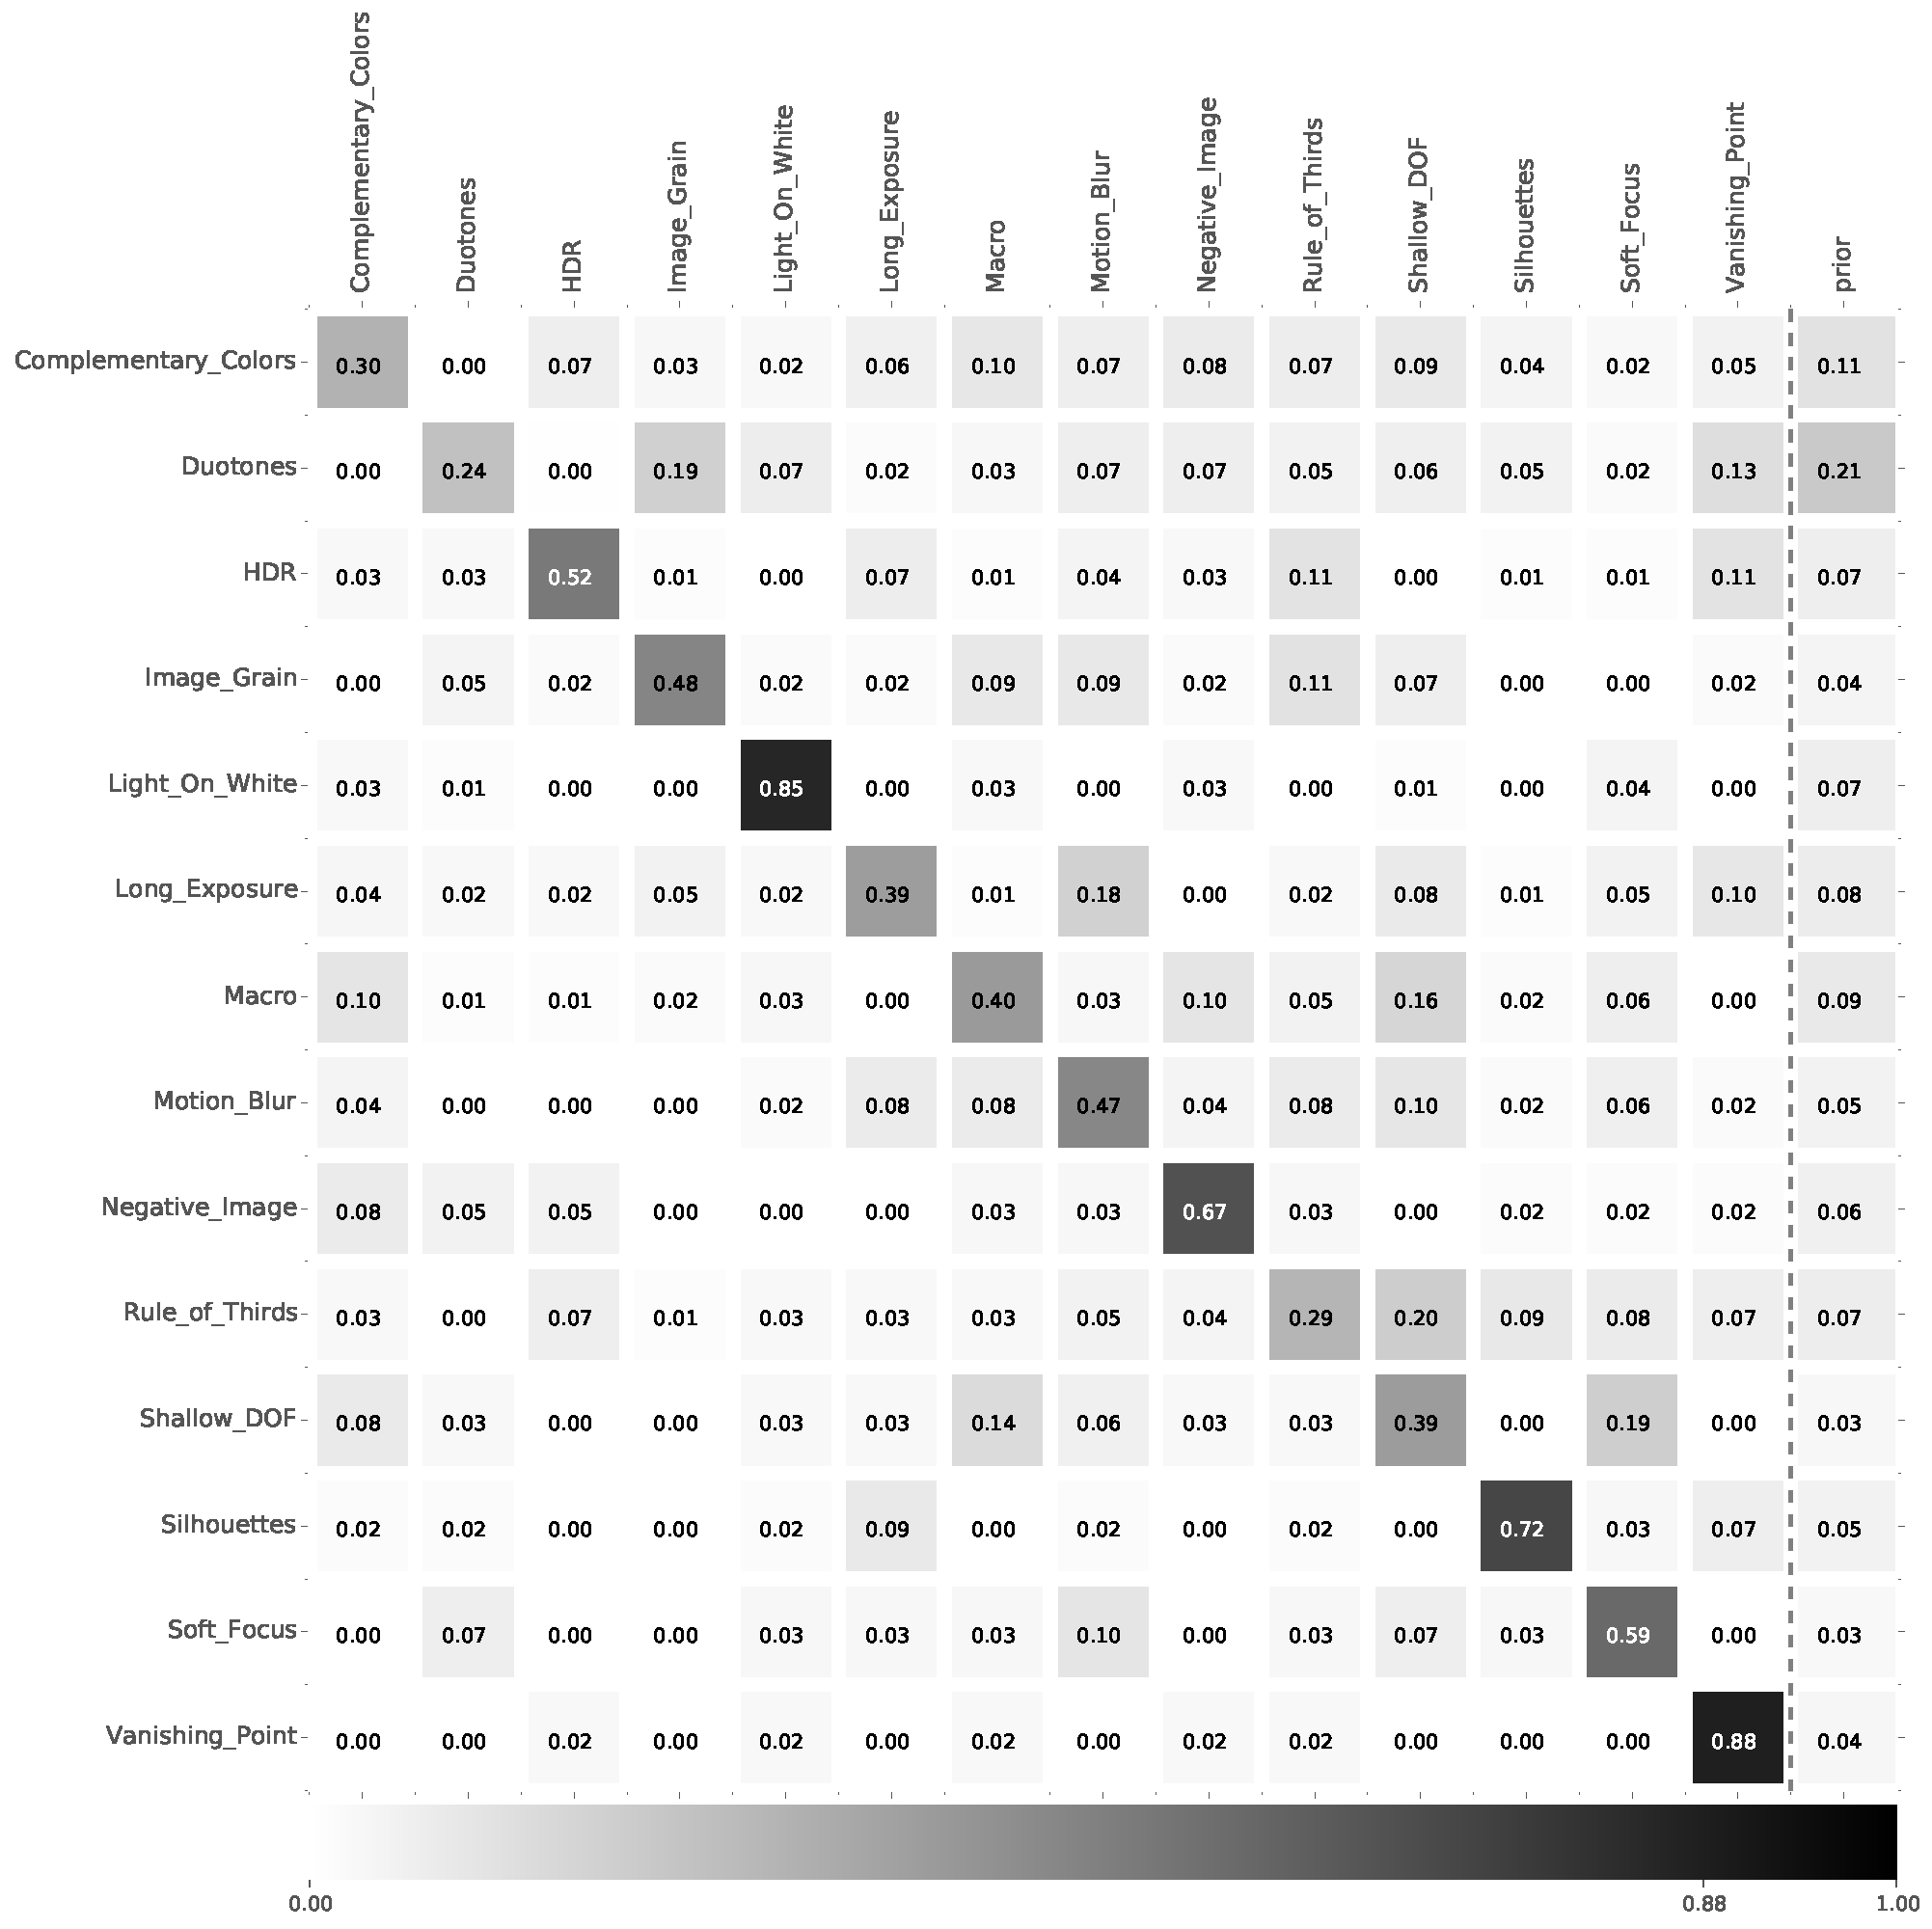
\includegraphics[width=\linewidth]{../style/figures/evaluation/ava_style_conf.pdf}
% \caption
% [Confusion matrix of our best classifier on the AVA Style dataset.]
% {
% Confusion matrix of our best classifier (\mbox{Late-fusion $\times$ Content}) on the AVA Style dataset.
% The right-most ``prior'' column reflects the distribution of ground-truth labels in the test set.
% The confusions are mostly understandable: ``Soft Focus'' vs. ``Motion Blur'' for example.
% }
% \label{fig:ava_style_conf}
% \end{figure*}

\begin{figure}
\centering
    \begin{tabular}{m{.01\linewidth} m{.16\linewidth} m{.16\linewidth} m{.16\linewidth} m{.16\linewidth} m{.16\linewidth}}
    \begin{turn}{90}{Horror}\end{turn} &
    \includegraphics[width=\linewidth]{../style/figures/flickr_on_flickr/pred_style_Horror/0.jpg} &
    \includegraphics[width=\linewidth]{../style/figures/flickr_on_flickr/pred_style_Horror/1.jpg} &
    \includegraphics[width=\linewidth]{../style/figures/flickr_on_flickr/pred_style_Horror/2.jpg} &
    \includegraphics[width=\linewidth]{../style/figures/flickr_on_flickr/pred_style_Horror/3.jpg} &
    \includegraphics[width=\linewidth]{../style/figures/flickr_on_flickr/pred_style_Horror/4.jpg} \\
    \begin{turn}{90}{Long Exposure}\end{turn} &
    \includegraphics[width=\linewidth]{../style/figures/flickr_on_flickr/pred_style_Long_Exposure/0.jpg} &
    \includegraphics[width=\linewidth]{../style/figures/flickr_on_flickr/pred_style_Long_Exposure/1.jpg} &
    \includegraphics[width=\linewidth]{../style/figures/flickr_on_flickr/pred_style_Long_Exposure/2.jpg} &
    \includegraphics[width=\linewidth]{../style/figures/flickr_on_flickr/pred_style_Long_Exposure/3.jpg} &
    \includegraphics[width=\linewidth]{../style/figures/flickr_on_flickr/pred_style_Long_Exposure/4.jpg} \\
    \begin{turn}{90}{Macro}\end{turn} &
    \includegraphics[width=\linewidth]{../style/figures/flickr_on_flickr/pred_style_Macro/0.jpg} &
    \includegraphics[width=\linewidth]{../style/figures/flickr_on_flickr/pred_style_Macro/1.jpg} &
    \includegraphics[width=\linewidth]{../style/figures/flickr_on_flickr/pred_style_Macro/2.jpg} &
    \includegraphics[width=\linewidth]{../style/figures/flickr_on_flickr/pred_style_Macro/3.jpg} &
    \includegraphics[width=\linewidth]{../style/figures/flickr_on_flickr/pred_style_Macro/4.jpg} \\
    \begin{turn}{90}{Melancholy}\end{turn} &
    \includegraphics[width=\linewidth]{../style/figures/flickr_on_flickr/pred_style_Melancholy/0.jpg} &
    \includegraphics[width=\linewidth]{../style/figures/flickr_on_flickr/pred_style_Melancholy/1.jpg} &
    \includegraphics[width=\linewidth]{../style/figures/flickr_on_flickr/pred_style_Melancholy/2.jpg} &
    \includegraphics[width=\linewidth]{../style/figures/flickr_on_flickr/pred_style_Melancholy/3.jpg} &
    \includegraphics[width=\linewidth]{../style/figures/flickr_on_flickr/pred_style_Melancholy/4.jpg} \\
    \begin{turn}{90}{Minimal}\end{turn} &
    \includegraphics[width=\linewidth]{../style/figures/flickr_on_flickr/pred_style_Minimal/0.jpg} &
    \includegraphics[width=\linewidth]{../style/figures/flickr_on_flickr/pred_style_Minimal/1.jpg} &
    \includegraphics[width=\linewidth]{../style/figures/flickr_on_flickr/pred_style_Minimal/2.jpg} &
    \includegraphics[width=\linewidth]{../style/figures/flickr_on_flickr/pred_style_Minimal/3.jpg} &
    \includegraphics[width=\linewidth]{../style/figures/flickr_on_flickr/pred_style_Minimal/4.jpg} \\
    \begin{turn}{90}{Noir}\end{turn} &
    \includegraphics[width=\linewidth]{../style/figures/flickr_on_flickr/pred_style_Noir/0.jpg} &
    \includegraphics[width=\linewidth]{../style/figures/flickr_on_flickr/pred_style_Noir/1.jpg} &
    \includegraphics[width=\linewidth]{../style/figures/flickr_on_flickr/pred_style_Noir/2.jpg} &
    \includegraphics[width=\linewidth]{../style/figures/flickr_on_flickr/pred_style_Noir/3.jpg} &
    \includegraphics[width=\linewidth]{../style/figures/flickr_on_flickr/pred_style_Noir/4.jpg}
\end{tabular}
\caption{
    Top five most confident predictions on the Flickr Style test set: styles 9-14.
}\label{fig:flickr_on_flickr2}
\end{figure}

\begin{figure}
\centering
    \begin{tabular}{m{.01\linewidth} m{.16\linewidth} m{.16\linewidth} m{.16\linewidth} m{.16\linewidth} m{.16\linewidth}}
    \begin{turn}{90}{Pastel}\end{turn} &
    \includegraphics[width=\linewidth]{../style/figures/flickr_on_flickr/pred_style_Pastel/0.jpg} &
    \includegraphics[width=\linewidth]{../style/figures/flickr_on_flickr/pred_style_Pastel/1.jpg} &
    \includegraphics[width=\linewidth]{../style/figures/flickr_on_flickr/pred_style_Pastel/2.jpg} &
    \includegraphics[width=\linewidth]{../style/figures/flickr_on_flickr/pred_style_Pastel/3.jpg} &
    \includegraphics[width=\linewidth]{../style/figures/flickr_on_flickr/pred_style_Pastel/4.jpg} \\
    \begin{turn}{90}{Romantic}\end{turn} &
    \includegraphics[width=\linewidth]{../style/figures/flickr_on_flickr/pred_style_Romantic/0.jpg} &
    \includegraphics[width=\linewidth]{../style/figures/flickr_on_flickr/pred_style_Romantic/1.jpg} &
    \includegraphics[width=\linewidth]{../style/figures/flickr_on_flickr/pred_style_Romantic/2.jpg} &
    \includegraphics[width=\linewidth]{../style/figures/flickr_on_flickr/pred_style_Romantic/3.jpg} &
    \includegraphics[width=\linewidth]{../style/figures/flickr_on_flickr/pred_style_Romantic/4.jpg} \\
    \begin{turn}{90}{Serene}\end{turn} &
    \includegraphics[width=\linewidth]{../style/figures/flickr_on_flickr/pred_style_Serene/0.jpg} &
    \includegraphics[width=\linewidth]{../style/figures/flickr_on_flickr/pred_style_Serene/1.jpg} &
    \includegraphics[width=\linewidth]{../style/figures/flickr_on_flickr/pred_style_Serene/2.jpg} &
    \includegraphics[width=\linewidth]{../style/figures/flickr_on_flickr/pred_style_Serene/3.jpg} &
    \includegraphics[width=\linewidth]{../style/figures/flickr_on_flickr/pred_style_Serene/4.jpg} \\
    \begin{turn}{90}{Sunny}\end{turn} &
    \includegraphics[width=\linewidth]{../style/figures/flickr_on_flickr/pred_style_Sunny/0.jpg} &
    \includegraphics[width=\linewidth]{../style/figures/flickr_on_flickr/pred_style_Sunny/1.jpg} &
    \includegraphics[width=\linewidth]{../style/figures/flickr_on_flickr/pred_style_Sunny/2.jpg} &
    \includegraphics[width=\linewidth]{../style/figures/flickr_on_flickr/pred_style_Sunny/3.jpg} &
    \includegraphics[width=\linewidth]{../style/figures/flickr_on_flickr/pred_style_Sunny/4.jpg} \\
    \begin{turn}{90}{Texture}\end{turn} &
    \includegraphics[width=\linewidth]{../style/figures/flickr_on_flickr/pred_style_Texture/0.jpg} &
    \includegraphics[width=\linewidth]{../style/figures/flickr_on_flickr/pred_style_Texture/1.jpg} &
    \includegraphics[width=\linewidth]{../style/figures/flickr_on_flickr/pred_style_Texture/2.jpg} &
    \includegraphics[width=\linewidth]{../style/figures/flickr_on_flickr/pred_style_Texture/3.jpg} &
    \includegraphics[width=\linewidth]{../style/figures/flickr_on_flickr/pred_style_Texture/4.jpg} \\
    \begin{turn}{90}{Vintage}\end{turn} &
    \includegraphics[width=\linewidth]{../style/figures/flickr_on_flickr/pred_style_Vintage/0.jpg} &
    \includegraphics[width=\linewidth]{../style/figures/flickr_on_flickr/pred_style_Vintage/1.jpg} &
    \includegraphics[width=\linewidth]{../style/figures/flickr_on_flickr/pred_style_Vintage/2.jpg} &
    \includegraphics[width=\linewidth]{../style/figures/flickr_on_flickr/pred_style_Vintage/3.jpg} &
    \includegraphics[width=\linewidth]{../style/figures/flickr_on_flickr/pred_style_Vintage/4.jpg}
\end{tabular}
\caption{
    Top five most confident predictions on the Flickr Style test set: styles 15-20.
}\label{fig:flickr_on_flickr3}
\end{figure}

\begin{table*}[ht!]
\caption{
    All per-class APs on all evaluated features on the Flickr dataset.
}\label{tab:flickr_ap_table}
\vspace{1em}
\centering
\begin{tabular}{llll}
\toprule
{}                     & Fusion x Content & DeCAF$_6$ & MC-bit \\
\midrule
Bokeh                  & 0.288            & 0.253     & 0.248 \\
Bright                 & 0.251            & 0.236     & 0.183 \\
Depth\_of\_Field       & 0.169            & 0.152     & 0.148 \\
Detailed               & 0.337            & 0.277     & 0.278 \\
Ethereal               & 0.408            & 0.393     & 0.335 \\
Geometric\_Composition & 0.411            & 0.355     & 0.360 \\
HDR                    & 0.487            & 0.406     & 0.475 \\
Hazy                   & 0.493            & 0.451     & 0.447 \\
Horror                 & 0.400            & 0.396     & 0.295 \\
Long\_Exposure         & 0.515            & 0.457     & 0.463 \\
Macro                  & 0.617            & 0.582     & 0.530 \\
Melancholy             & 0.168            & 0.147     & 0.136 \\
Minimal                & 0.512            & 0.444     & 0.481 \\
Noir                   & 0.494            & 0.481     & 0.408 \\
Pastel                 & 0.258            & 0.245     & 0.211 \\
Romantic               & 0.227            & 0.204     & 0.185 \\
Serene                 & 0.281            & 0.257     & 0.239 \\
Sunny                  & 0.500            & 0.481     & 0.453 \\
Texture                & 0.265            & 0.227     & 0.229 \\
Vintage                & 0.282            & 0.273     & 0.222 \\
\midrule
mean                   & 0.368            & 0.336     & 0.316 \\
\bottomrule
\end{tabular}
\end{table*}

\begin{table*}[ht!]
\caption{Comparison of Flickr Style per-class accuracies for our method and Mech Turkers.}\label{tab:flickr_vs_mturk}
\centering
\small{
\begin{tabular}{rccc}
\toprule
{}                    & MTurk acc., Flickr g.t. & Our acc., Flickr g.t. & Our acc., MTurk g.t. \\
\midrule
Bright                & 69.10                       & 73.38                     & 73.63 \\
Depth of Field        & 68.92                       & 68.50                     & 81.05 \\
Detailed              & 65.47                       & 75.25                     & 68.44 \\
Ethereal              & 76.92                       & 80.62                     & 77.95 \\
Geometric Composition & 81.52                       & 77.75                     & 80.31 \\
HDR                   & 71.84                       & 82.00                     & 76.96 \\
Hazy                  & 83.49                       & 80.75                     & 81.64 \\
Horror                & 89.85                       & 84.25                     & 81.64 \\
Long Exposure         & 73.12                       & 84.19                     & 76.79 \\
Macro                 & 92.25                       & 86.56                     & 88.39 \\
Melancholy            & 67.77                       & 70.88                     & 71.25 \\
Minimal               & 79.71                       & 83.75                     & 78.57 \\
Noir                  & 81.35                       & 85.25                     & 85.88 \\
Pastel                & 66.94                       & 74.56                     & 75.47 \\
Romantic              & 60.91                       & 68.00                     & 66.25 \\
Serene                & 69.49                       & 70.44                     & 76.80 \\
Sunny                 & 84.48                       & 84.56                     & 79.94 \\
Vintage               & 68.77                       & 75.50                     & 67.80 \\
\midrule
Mean                  & 75.11                       & 78.12                     & 77.15 \\
\end{tabular}
}
\end{table*}

\begin{table*}[ht!]
\caption{Signficant deviations between human and machine accuracies on Flickr Style.}\label{tab:flickr_vs_mturk2}
\centering
\small{
\begin{tabular}{rccc}
\toprule
{}                    & Our acc., Flickr g.t.   & Our acc., MTurk g.t.  & \% change from Flickr to MTurk g.t. \\
\midrule
Vintage               & 75.50                       & 67.80                     & -10.19 \\
Detailed              & 75.25                       & 68.44                     & -9.05 \\
Long Exposure         & 84.19                       & 76.79                     & -8.79 \\
Minimal               & 83.75                       & 78.57                     & -6.18 \\
HDR                   & 82.00                       & 76.96                     & -6.15 \\
Sunny                 & 84.56                       & 79.94                     & -5.46 \\
Serene                & 70.44                       & 76.80                     & 9.03 \\
Depth of Field        & 68.50                       & 81.05                     & 18.32 \\
\toprule
{}                     & Our acc., Flickr g.t. & MTurk acc., Flickr g.t. & Acc. difference \\
\midrule
Horror                 & 84.25                     & 90.42                       & -6.17 \\
Macro                  & 86.56                     & 91.71                       & -5.15 \\
Romantic               & 68.00                     & 61.04                       & 6.96 \\
Pastel                 & 74.56                     & 66.87                       & 7.69 \\
HDR                    & 82.00                     & 72.79                       & 9.21 \\
Long Exposure          & 84.19                     & 73.83                       & 10.35 \\
Detailed               & 75.25                     & 63.30                       & 11.95 \\
\end{tabular}
}
\end{table*}

\begin{figure*}[ht!]
\centering
\includegraphics[width=1\linewidth]{../style/figures/evaluation/flickr_conf.pdf}
\caption
[Confusion matrix of our best classifier on the Flickr dataset.]
{Confusion matrix of our best classifier (\mbox{Late-fusion $\times$ Content}) on the Flickr dataset.}
\label{fig:flickr_conf}
\end{figure*}

\begin{table*}[ht!]
\centering
\caption{
    All per-class APs on all evaluated features on the Wikipaintings dataset.
}\label{tab:wikipaintings_ap_table}
\vspace{1em}
\begin{tabular}{llllll}
\toprule
{}                             & Fusion x Content & MC-bit & DeCAF$_6$  \\
\midrule
Abstract\_Art                  & 0.341            & 0.314  & 0.258      \\
Abstract\_Expressionism        & 0.351            & 0.340  & 0.243      \\
Art\_Informel                  & 0.221            & 0.217  & 0.187      \\
Art\_Nouveau\_(Modern)         & 0.421            & 0.402  & 0.197      \\
Baroque                        & 0.436            & 0.386  & 0.313      \\
Color\_Field\_Painting         & 0.773            & 0.739  & 0.689      \\
Cubism                         & 0.495            & 0.488  & 0.400      \\
Early\_Renaissance             & 0.578            & 0.559  & 0.453      \\
Expressionism                  & 0.235            & 0.230  & 0.186      \\
High\_Renaissance              & 0.401            & 0.345  & 0.288      \\
Impressionism                  & 0.586            & 0.528  & 0.411      \\
Magic\_Realism                 & 0.521            & 0.465  & 0.428      \\
Mannerism\_(Late\_Renaissance) & 0.505            & 0.439  & 0.356      \\
Minimalism                     & 0.660            & 0.614  & 0.604      \\
Nave\_Art\_(Primitivism)       & 0.395            & 0.425  & 0.225      \\
Neoclassicism                  & 0.601            & 0.537  & 0.399      \\
Northern\_Renaissance          & 0.560            & 0.478  & 0.433      \\
Pop\_Art                       & 0.441            & 0.398  & 0.281      \\
Post-Impressionism             & 0.348            & 0.348  & 0.292      \\
Realism                        & 0.408            & 0.309  & 0.266      \\
Rococo                         & 0.616            & 0.548  & 0.467      \\
Romanticism                    & 0.392            & 0.389  & 0.343      \\
Surrealism                     & 0.262            & 0.247  & 0.134      \\
Symbolism                      & 0.390            & 0.390  & 0.260      \\
Ukiyo-e                        & 0.895            & 0.894  & 0.788      \\
\midrule
mean                           & 0.473            & 0.441  & 0.356      \\
\bottomrule
\end{tabular}
\end{table*}

\begin{table*}
\caption{
    Per-class accuracies on the Wikipaintings dataset, using the MC-bit feature.
}\label{tab:wp_accuracies}
\vspace{1em}
\centering
\begin{tabular}{lrlr}
\toprule
\textbf{Style} & \textbf{Accuracy} & \textbf{Style} & \textbf{Accuracy} \\
\midrule
Symbolism                    &         71.24 & Impressionism                &         82.15 \\
Expressionism                &         72.03 & Northern Renaissance         &         82.32 \\
Art Nouveau (Modern)         &         72.77 & High Renaissance             &         82.90 \\
Nave Art (Primitivism)       &         72.95 & Mannerism (Late Renaissance) &         83.04 \\
Surrealism                   &         74.44 & Pop Art                      &         83.33 \\
Post-Impressionism           &         74.51 & Early Renaissance            &         84.69 \\
Romanticism                  &         75.86 & Abstract Art                 &         85.10 \\
Realism                      &         75.88 & Cubism                       &         86.85 \\
Magic Realism                &         78.54 & Rococo                       &         87.33 \\
Neoclassicism                &         80.18 & Ukiyo-e                      &         93.18 \\
Abstract Expressionism       &         81.25 & Minimalism                   &         94.21 \\
Baroque                      &         81.45 & Color Field Painting         &         95.58 \\
Art Informel                 &         82.09 &                              &               \\
\bottomrule
\end{tabular}
\end{table*}

\begin{figure*}[ht!]
\centering
\includegraphics[width=1\linewidth]{../style/figures/evaluation/wikipaintings_conf.pdf}
\caption
[Confusion matrix of our best classifier on the Wikipaintings dataset.]
{Confusion matrix of our best classifier (\mbox{Late-fusion $\times$ Content}) on the Wikipaintings dataset.}
\label{fig:wp_conf}
\end{figure*}

% \begin{figure}[th]
% \centering
% \includegraphics[width=\linewidth]{../style/figures/wikipaintings_style.pdf}\\
% \includegraphics[width=\linewidth]{../style/figures/wikipaintings_genre.pdf}\\
% \includegraphics[width=\linewidth]{../style/figures/wikipaintings_date.pdf}
% \caption{Distribution of image style, genre, and date in the Wikipaintings dataset.}
% \label{fig:wikipaintings_data}
% \end{figure}



%================================
\printbibliography
\end{document}
